%%%%%%%%%%%%%%%%%%%%%%%%%%%%%%%%%%%%%%%%%%%%%%%%%%%%%%%%%%%%%%%%%%%%%%%%%
%  Content: Main file of thesis template (master/enginering).
%  Author: Tomasz Kubik <tomasz.kubik@pwr.edu.pl>
%  Data: 1 marca 2020
%  Wersja: 0.4
%%%%%%%%%%%%%%%%%%%%%%%%%%%%%%%%%%%%%%%%%%%%%%%%%%%%%%%%%%%%%%%%%%%%%%%%%

\documentclass[a4paper,onecolumn,12pt,twoside,extrafontsizes]{memoir}
% In order to prepare the manuscript for archives (2x1, double printed) you can:
% a) produce normal pdf, then convert it to pdf with two pages on one phisical page (solution suggested)
%
%   This can be done by:
%   - printing from Adobe Acrobat Reader with option "Multiple"
%   - using psutils
%
%      Windows (assuming that you have MiKTeX installed with the package pakiet miktex-psutils-bin-x64-2.9):
%        "c:\Program Files\MiKTeX 2.9\miktex\bin\x64\pdf2ps.exe" Dyplom.pdf Dyplom.ps 
%        "c:\Program Files\MiKTeX 2.9\miktex\bin\x64\psnup.exe" -2 Dyplom.ps Dyplom2.ps
%        "c:\Program Files\MiKTeX 2.9\miktex\bin\x64\ps2pdf.exe" Dyplom2.ps Dyplom2.pdf
%        Del Dyplom2.ps Dyplom.ps
%
%     Linux:
%        pdf2ps Dyplom.pdf - | psnup -2 | ps2pdf - Dyplom2.pdf
%
%
% b) produce 'reduced' pdf by settning smaller fonts in the document class definition (it changes the formating thus it is not suggested)
%
%   Use of the following commands instead of original one:
%   \documentclass[a4paper,onecolumn,twoside,10pt]{memoir} 
%   \renewcommand{\normalsize}{\fontsize{8pt}{10pt}\selectfont}

%\usepackage[cp1250]{inputenc} % for cp1250 file encoding
\usepackage{amssymb}
\usepackage{emptypage}

\usepackage[utf8]{inputenc} % for UTF8 file encoding
\usepackage[T1]{fontenc}
\usepackage[polish]{babel}
%\usepackage[english]{babel}
%\DisemulatePackage{setspace}
\usepackage{setspace}
\usepackage{tabularx}
\usepackage{color,calc}
\usepackage{threeparttable,tablefootnote}

%\usepackage{soul} % packege with commands for text highliting

%% Accorging to the rules the main font of the thesis should be Times.
%% In order to achieve it we use tgtermes font that offers shapes: normal, bold, italic, italic bold.
%% There is no slanted shape.
%% If you use slanted font in the text (typing \textsl{} commnand), then LaTeX will substitute it with a standard font giving you a warning.
%% Additionally tgtermes works for the running text. All maths (formulas, equations) will be rendered with a default font for math.
%% If you with to change the font for math, you must to do it yourself.

%% After installation of tgtermes package there might be a need to update font and mapping information 
%% This can be don by running the following commands (as administrator)
%% initexmf --admin --update-fndb
%% initexmf --admin --mkmaps

\usepackage{tgtermes}   

\renewcommand*\ttdefault{txtt}

% The settings regarding fonts were used in the earlier version of the template. It is kept for historical reasons
%\usepackage{mathptmx} 
%\usepackage{newtxtext,newtxmath} 
%\usepackage{newtxmath,tgtermes} 

\usepackage{listings} % used to render the source code 
% In UTF8 encoding there was a need to define the following mapping (otherwise the national characters were not recognized correctly)
%%\lstset{literate=%-
%%{ą}{{\k{a}}}1 {ć}{{\'c}}1 {ę}{{\k{e}}}1 {ł}{{\l{}}}1 {ń}{{\'n}}1 {ó}{{\'o}}1 {ś}{{\'s}}1 {ż}{{\.z}}1 {ź}{{\'z}}1 {Ą}{{\k{A}}}1 {Ć}{{\'C}}1 {Ę}{{\k{E}}}1 {Ł}{{\L{}}}1 {Ń}{{\'N}}1 {Ó}{{\'O}}1 {Ś}{{\'S}}1 {Ż}{{\.Z}}1 {Ź}{{\'Z}}1 
    %%{Ö}{{\"O}}1
    %%{Ä}{{\"A}}1
    %%{Ü}{{\"U}}1
    %%{ß}{{\ss}}1
    %%{ü}{{\"u}}1
    %%{ä}{{\"a}}1
    %%{ö}{{\"o}}1
    %%{~}{{\textasciitilde}}1
		%%{—}{{{\textemdash} }}1
%%}%{\ \ }{{\ }}1}

\usepackage{pgfplots}

\usepackage{amsmath}
\usepackage{multicol}
\usepackage{placeins}
\usepackage{makecell}

\usepackage{siunitx}
\usepackage{physics}
\usepackage[f]{esvect}
\newcommand{\normalize}[1]{
  \ensuremath{\frac{#1}{\Vert#1\Vert}}
}
\newcommand{\length}[1]{
  \ensuremath{\Vert#1\Vert}
}

\usepackage{tikz}
\usetikzlibrary{quotes,babel,calc,patterns,angles, arrows.meta, intersections}
 \usepackage{pdfpages}
 \usepackage{wrapfig}
 \usepackage{pifont}

 \usepackage{float}
 \usepackage{longtable}
 \usepackage{xltabular}
 \usepackage{eqexpl}

 \newcommand{\cmark}{\ding{51}}%
\newcommand{\xmark}{\ding{55}}%

 \eqexplSetIntro{gdzie:}
% \usepackage{mathdots}
% \usepackage{yhmath}
% \usepackage{cancel}
% \usepackage{color}
% \usepackage{siunitx}
% \usepackage{array}
% \usepackage{multirow}
% \usepackage{amssymb}
% \usepackage{gensymb}
% \usepackage{tabularx}
% \usepackage{booktabs}
% \usetikzlibrary{patterns}
% \usetikzlibrary{shadows.blur}
% \usetikzlibrary{shapes}



\newcommand{\listingcaption}[1]% added to handle captions of listings in two columns 
{%
\vspace*{\abovecaptionskip}\small 
\refstepcounter{lstlisting}\hfill%
Listing \thelstlisting: #1\hfill%\hfill%
\addcontentsline{lol}{lstlisting}{\protect\numberline{\thelstlisting}#1}
}%

\lstdefinelanguage{JavaScript}{
  keywords={typeof, new, true, false, catch, function, return, null, catch, switch, var, if, in, while, do, else, case, break},
  keywordstyle=\color{blue}\bfseries,
  ndkeywords={class, export, boolean, default, extends throw, implements, import, this, void, number, string, public, private, protected, extends, from, constructor},
  ndkeywordstyle=\color{darkgray}\bfseries,
  identifierstyle=\color{black},
  sensitive=false,
  comment=[l]{//},
  morecomment=[s]{/*}{*/},
  commentstyle=\color{purple}\ttfamily,
  stringstyle=\color{red}\ttfamily,
  morestring=[b]',
  morestring=[b]"
}

% code style with line numbering (but these are commented out)
\lstset{
  basicstyle=\footnotesize\ttfamily,
  %%columns=fullflexible,
	%%showstringspaces=false,
	%%showspaces=false,
  breaklines=true,
  postbreak=\mbox{\textcolor{red}{$\hookrightarrow$}\space},
  %%numbers=left,
  %%firstnumber=1,
  %%numberfirstline=true,
	%%xleftmargin=17pt,
  %%framexleftmargin=17pt,
  %%framexrightmargin=5pt,
  %%framexbottommargin=4pt,
	belowskip=.5\baselineskip
}

% code style without line numbering
%%\lstset{
  %%basicstyle=\footnotesize\ttfamily,
  %%columns=fullflexible,
	%%showstringspaces=false,
	%%showspaces=false,
  %%breaklines=true,
  %%postbreak=\mbox{\textcolor{red}{$\hookrightarrow$}\space},
%%}

%% Here you have another example of code styling
%%\lstloadlanguages{% Check Dokumentation for further languages ...
%%C,
%%C++,
%%csh,
%%Java
%%}
%%
%%\definecolor{red}{rgb}{0.6,0,0} % for strings
%%\definecolor{blue}{rgb}{0,0,0.6}
%%\definecolor{green}{rgb}{0,0.8,0}
%%\definecolor{cyan}{rgb}{0.0,0.6,0.6}
%%
%%\lstdefinestyle{sqlstyle}{
%%language=SQL,
%%basicstyle=\footnotesize\ttfamily, 
%%numbers=left, 
%%numberstyle=\tiny, 
%%numbersep=5pt, 
%%tabsize=2, 
%%extendedchars=true, 
%%breaklines=true, 
%%showspaces=false, 
%%showtabs=true, 
%%xleftmargin=17pt,
%%framexleftmargin=17pt,
%%framexrightmargin=5pt,
%%framexbottommargin=4pt,
%%keywordstyle=\color{blue}, 
%%commentstyle=\color{green}, 
%%stringstyle=\color{red}, 
%%}
%%
%%\lstdefinestyle{sharpcstyle}{
%%language=[Sharp]C,
%%basicstyle=\footnotesize\ttfamily, 
%%numbers=left, 
%%numberstyle=\tiny, 
%%numbersep=5pt, 
%%tabsize=2, 
%%extendedchars=true, 
%%breaklines=true, 
%%showspaces=false, 
%%showtabs=true, 
%%xleftmargin=17pt,
%%framexleftmargin=17pt,
%%framexrightmargin=5pt,
%%framexbottommargin=4pt,
%%morecomment=[l]{//}, %use comment-line-style!
%%morecomment=[s]{/*}{*/}, %for multiline comments
%%showstringspaces=false, 
%%morekeywords={  abstract, event, new, struct,
                %%as, explicit, null, switch,
                %%base, extern, object, this,
                %%bool, false, operator, throw,
                %%break, finally, out, true,
                %%byte, fixed, override, try,
                %%case, float, params, typeof,
                %%catch, for, private, uint,
                %%char, foreach, protected, ulong,
                %%checked, goto, public, unchecked,
                %%class, if, readonly, unsafe,
                %%const, implicit, ref, ushort,
                %%continue, in, return, using,
                %%decimal, int, sbyte, virtual,
                %%default, interface, sealed, volatile,
                %%delegate, internal, short, void,
                %%do, is, sizeof, while,
                %%double, lock, stackalloc,
                %%else, long, static,
                %%enum, namespace, string},
%%keywordstyle=\color{cyan},
%%identifierstyle=\color{red},
%%stringstyle=\color{blue}, 
%%commentstyle=\color{green},
%%}


\renewcommand\lstlistlistingname{Spis listingów}
\makeatletter
%\renewcommand*{\l@lstlisting}[2]{\@dottedtocline{1}{0em}{2.3em}{#1}{#2}}
\g@addto@macro\insertchapterspace{\addtocontents{lol}{\protect\addvspace{10pt}}}
\renewcommand*{\l@lstlisting}{\@dottedtocline{1}{0em}{2.3em}}
\makeatother

\renewcommand*{\lstlistlistingname}{Spis listingów} \newlistof{lstlistoflistings}{lol}{\lstlistlistingname}



% It is possible to use packages mentioned below for making various tables but it is suggested to left them unused
%\usepackage{longtable}
%\usepackage{ltxtable}
%\usepackage{tabulary}

%%%%%%%%%%%%%%%%%%%%%%%%%%%%%%%%%%%%%%%%%%%%%%%%%%%
%% Settings related to the autmatic document typesetting
%% and floats placements
%%%%%%%%%%%%%%%%%%%%%%%%%%%%%%%%%%%%%%%%%%%%%%%%%%%
%\hyphenpenalty=10000		% do not break words too often
\clubpenalty=10000      % penalty for orphans
\widowpenalty=10000  % do not left widows
%\brokenpenalty=10000		% dont break words between pages - commented out because interfere with line breaking in lstlisting
%\exhyphenpenalty=999999		% dont break word with dash - commented out because interfere with line breaking in lstlisting
\righthyphenmin=3			% break at min 3 characters

%\tolerance=4500
%\pretolerance=250
%\hfuzz=1.5pt
%\hbadness=1450

\renewcommand{\topfraction}{0.95}
\renewcommand{\bottomfraction}{0.95}
\renewcommand{\textfraction}{0.05}
\renewcommand{\floatpagefraction}{0.35}

%%%%%%%%%%%%%%%%%%%%%%%%%%%%%%%%%%%%%%%%%%%%%%%%%%%
%%  Size settings: text, header and footer, marigins
%%  for documents based on memoir class
%%%%%%%%%%%%%%%%%%%%%%%%%%%%%%%%%%%%%%%%%%%%%%%%%%%
\setlength{\headsep}{10pt} 
\setlength{\headheight}{13.6pt} % baselineskip for 11pt font, i.e. \small, equals 13.6pt
\setlength{\footskip}{\headsep+\headheight}
\setlength{\uppermargin}{\headheight+\headsep+1cm}
\setlength{\textheight}{\paperheight-\uppermargin-\footskip-1.5cm}
\setlength{\textwidth}{\paperwidth-5cm}
\setlength{\spinemargin}{2.5cm}
\setlength{\foremargin}{2.5cm}
\setlength{\marginparsep}{2mm}
\setlength{\marginparwidth}{2.3mm}
%\settrimmedsize{297mm}{210mm}{*}
%\settrims{0mm}{0mm}	
\checkandfixthelayout[fixed] % needed to fix the layout
%%%%%%%%%%%%%%%%%%%%%%%%%%%%%%%%%%%%%%%%%%%%%%%%
%%  Settings related to the interline spaces, indentations, distances
%%%%%%%%%%%%%%%%%%%%%%%%%%%%%%%%%%%%%%%%%%%%%%%%
\linespread{1}
%\linespread{1.241}
\setlength{\parindent}{14.5pt}
%\setlength{\cftbeforechapterskip}{0.3em} % spaces in the table of contents
%\setbeforesecskip{10pt plus 0.5ex}%{-3.5ex \@plus -1ex \@minus -.2ex}
%\setaftersecskip{10pt plus 0.5ex}%\onelineskip}
%\setbeforesubsecskip{8pt plus 0.5ex}%{-3.5ex \@plus -1ex \@minus -.2ex}
%\setaftersubsecskip{8pt plus 0.5ex}%\onelineskip}
%\setlength\floatsep{6pt plus 2pt minus 2pt} 
%\setlength\intextsep{12pt plus 2pt minus 2pt} 
%\setlength\textfloatsep{12pt plus 2pt minus 2pt} 

%%%%%%%%%%%%%%%%%%%%%%%%%%%%%%%%%%%%%%%%%%%%%%%%%%%
%%  Pakiety i komendy zastosowane tylko do zamieszczenia informacji o użytych komendach i fontach
%%  Normalnie nie są potrzebne, można je zamarkować podczas redakcji pracy
%%%%%%%%%%%%%%%%%%%%%%%%%%%%%%%%%%%%%%%%%%%%%%%%%%%
\usepackage{./packages/memlays}     % extra layout diagrams, used only in template for 'debugging'. Is uses layouts package. Comment out them both if you edit your thesis
%\usepackage{layouts}
\usepackage{printlen} % allows displeying the values of defined lengths, used onlu in template for 'debugging'. Comment out it if you edit your thesis
\uselengthunit{pt}
\makeatletter
\newcommand{\showFontSize}{\f@size pt} % makro wypisujące wielkość bieżącej czcionki
\makeatother
% if you wish to show the frames:
%\usepackage{showframe} 


%%%%%%%%%%%%%%%%%%%%%%%%%%%%%%%%%%%%%%%%%%%%%%%%%%%
%%  Enumerated lists definitions
%%%%%%%%%%%%%%%%%%%%%%%%%%%%%%%%%%%%%%%%%%%%%%%%%%%

% Item lists have, by default, the bullets which are charactes not existing in the set of tgtermes fonts
% Therefore these are substituted by LaTeX with characters from standard set of fonts. In order to change this
% behavior you cad declare substitutions as below
%    \DeclareTextCommandDefault{\textbullet}{\ensuremath{\bullet}}
%    \DeclareTextCommandDefault{\textasteriskcentered}{\ensuremath{\ast}}
%    \DeclareTextCommandDefault{\textperiodcentered}{\ensuremath{\cdot}}
% But the better way is to redefine enumitem environment from enumitem package
\usepackage{enumitem}
\setlist{noitemsep,topsep=4pt,parsep=0pt,partopsep=4pt,leftmargin=*} % this makes list more compact
\setenumerate{labelindent=0pt,itemindent=0pt,leftmargin=!,label=\arabic*.} % it is possible to use \arabic or \alph, if the enumerations are supposed to be rendered with different numbers
\setlistdepth{4} % limits the depth of nested enumeration
\setlist[itemize,1]{label=$\bullet$}  % here we define the bullet at each of the levels
\setlist[itemize,2]{label=\normalfont\bfseries\textendash}
\setlist[itemize,3]{label=$\ast$}
\setlist[itemize,4]{label=$\cdot$}
\renewlist{itemize}{itemize}{4}

%%%http://tex.stackexchange.com/questions/29322/how-to-make-enumerate-items-align-at-left-margin
%\renewenvironment{enumerate}
%{
%\begin{list}{\arabic{enumi}.}
%{
%\usecounter{enumi}
%%\setlength{\itemindent}{0pt}
%%\setlength{\leftmargin}{1.8em}%{2zw} % 
%%\setlength{\rightmargin}{0zw} %
%%\setlength{\labelsep}{1zw} %
%%\setlength{\labelwidth}{3zw} % 
%\setlength{\topsep}{6pt}%
%\setlength{\partopsep}{0pt}%
%\setlength{\parskip}{0pt}%
%\setlength{\parsep}{0em} % 
%\setlength{\itemsep}{0em} % 
%%\setlength{\listparindent}{1zw} % 
%}
%}{
%\end{list}
%}

\makeatletter
\renewenvironment{quote}{
	\begin{list}{}
	{
	\setlength{\leftmargin}{1em}
	\setlength{\topsep}{0pt}%
	\setlength{\partopsep}{0pt}%
	\setlength{\parskip}{0pt}%
	\setlength{\parsep}{0pt}%
	\setlength{\itemsep}{0pt}
	}
	}{
	\end{list}}
\makeatother

%%%%%%%%%%%%%%%%%%%%%%%%%%%%%%%%%%%%%%%%%
%%  Package for index generation (must be set before hyperref)
%%%%%%%%%%%%%%%%%%%%%%%%%%%%%%%%%%%%%%%%%
%%\DisemulatePackage{imakeidx} % uncomment it out if you wish to generate an index
%%\usepackage[makeindex,noautomatic]{imakeidx} % here we say that the index can not be generated automatically

\makeatletter
%%%\renewenvironment{theindex}
							 %%%{\vskip 10pt\@makeschapterhead{\indexname}\vskip -3pt%
								%%%\@mkboth{\MakeUppercase\indexname}%
												%%%{\MakeUppercase\indexname}%
								%%%\vspace{-3.2mm}\parindent\z@%
								%%%\renewcommand\subitem{\par\hangindent 16\p@ \hspace*{0\p@}}%%
								%%%\phantomsection%
								%%%\begin{multicols}{2}
								%%%%\thispagestyle{plain}
								%%%\parindent\z@                
								%%%%\parskip\z@ \@plus .3\p@\relax
								%%%\let\item\@idxitem}
							 %%%{\end{multicols}\clearpage}
%%%
\makeatother


\usepackage{ifpdf}
%\newif\ifpdf \ifx\pdfoutput\undefined
%\pdffalse % we are not running PDFLaTeX
%\else
%\pdfoutput=1 % we are running PDFLaTeX
%\pdftrue \fi
\ifpdf
 \usepackage[pdftex,bookmarks,breaklinks,unicode]{hyperref}
% \usepackage[pdftex]{graphicx}
 \DeclareGraphicsExtensions{.pdf,.jpg,.mps,.png}
\pdfcompresslevel=9
\pdfoutput=1
\makeatletter
\AtBeginDocument{  % Here are the metadata that will be embedded in the resulting pdf. Please fill in them correctly
  \hypersetup{
	pdfinfo={
    Title = {\@title},
    Author = {\@author},
    Subject={},
    Keywords={keywords},  
		Producer={},
		Creator={pdftex}
	}}
}
\pdftrailerid{} %Remove ID
\pdfsuppressptexinfo15 %Suppress PTEX.Fullbanner and info of imported PDFs

\makeatother
\else
\usepackage{graphicx}
\DeclareGraphicsExtensions{.eps,.ps,.jpg,.mps,.png}
\fi
\sloppy

%\graphicspath{{figures01/}{figures02/}} %% if you with to have set the paths to figures  


% Depth of numbering
\setcounter{secnumdepth}{2}
\setcounter{tocdepth}{2}
\setsecnumdepth{subsection} % activating subsubsec numbering in doc


% dots aftes sections numbers
\makeatletter
\def\@seccntformat#1{\csname the#1\endcsname.\quad}
\def\numberline#1{\hb@xt@\@tempdima{#1\if&#1&\else.\fi\hfil}}
\makeatother

\renewcommand{\chapternumberline}[1]{#1.\quad}
\renewcommand{\cftchapterdotsep}{\cftdotsep}

%\definecolor{niceblue}{rgb}{.168,.234,.671}

% Fonts in figures and tables captions
\captionnamefont{\small}
\captiontitlefont{\small}
% macro adjusting the way the chapter title is rendered
%\def\printchaptertitle##1{\fonttitle \space \thechapter.\space ##1} 

%\usepackage{ltcaption}
% The ltcaption package supports \CaptionLabelFont & \CaptionTextFont introduced by the NTG document classes
%\renewcommand\CaptionLabelFont{\small}
%\renewcommand\CaptionTextFont{\small}

% Redefinitions of labels for tables, figures and bibliography 
%\AtBeginDocument{% 
        \addto\captionspolish{% 
        \renewcommand{\tablename}{Tab.}% 
}%} 

%\AtBeginDocument{% 
%        \addto\captionspolish{% 
%        \renewcommand{\chaptername}{Rozdział}% 
%}} 

%\AtBeginDocument{% 
        \addto\captionspolish{% 
        \renewcommand{\figurename}{Rys.}% 
}%}


%\AtBeginDocument{% 
        \addto\captionspolish{% 
        \renewcommand{\bibname}{Literatura}% 
}%}

%\AtBeginDocument{% 
        \addto\captionspolish{% 
        \renewcommand{\listfigurename}{Spis rysunków}% 
}%}

%\AtBeginDocument{% 
        \addto\captionspolish{% 
        \renewcommand{\listtablename}{Spis tabel}% 
}%}

%\AtBeginDocument{% 
        \addto\captionspolish

%%%%%%%%%%%%%%%%%%%%%%%%%%%%%%%%%%%%%%%%%%%%%%%%%%%%%%%%%%%%%%%%%%                  
%% Definition of headers and footers appearing on pages
%%%%%%%%%%%%%%%%%%%%%%%%%%%%%%%%%%%%%%%%%%%%%%%%%%%%%%%%%%%%%%%%%%                  
\addtopsmarks{headings}{%
\nouppercaseheads % added at the beginning
}{%
\createmark{chapter}{both}{shownumber}{}{. \space}
%\createmark{chapter}{left}{shownumber}{}{. \space}
\createmark{section}{right}{shownumber}{}{. \space}
}%use the new settings

\makeatletter
\copypagestyle{outer}{headings}
\makeoddhead{outer}{}{}{\small\itshape\rightmark}
\makeevenhead{outer}{\small\itshape\leftmark}{}{}
\makeoddfoot{outer}{\small\@author:~\@titleShort}{}{\small\thepage}
\makeevenfoot{outer}{\small\thepage}{}{\small\@author:~\@titleShort}
\makeheadrule{outer}{\linewidth}{\normalrulethickness}
\makefootrule{outer}{\linewidth}{\normalrulethickness}{2pt}
\makeatother

% fix plain
\copypagestyle{plain}{headings} % overwrite plain with outer
\makeoddhead{plain}{}{}{} % remove right header
\makeevenhead{plain}{}{}{} % remove left header
\makeevenfoot{plain}{}{}{}
\makeoddfoot{plain}{}{}{}

\copypagestyle{empty}{headings} % overwrite plain with outer
\makeoddhead{empty}{}{}{} % remove right header
\makeevenhead{empty}{}{}{} % remove left header
\makeevenfoot{empty}{}{}{}
\makeoddfoot{empty}{}{}{}


%%%%%%%%%%%%%%%%%%%%%%%%%%%%%%%%%%%%%%%
%% Definition of title page
%%%%%%%%%%%%%%%%%%%%%%%%%%%%%%%%%%%%%%%
\makeatletter
% University
\newcommand\uczelnia[1]{\renewcommand\@uczelnia{#1}}
\newcommand\@uczelnia{}
% Faculty
\newcommand\wydzial[1]{\renewcommand\@wydzial{#1}}
\newcommand\@wydzial{}
% Field
\newcommand\kierunek[1]{\renewcommand\@kierunek{#1}}
\newcommand\@kierunek{}
% Speciality
\newcommand\specjalnosc[1]{\renewcommand\@specjalnosc{#1}}
\newcommand\@specjalnosc{}
% Title in english
\newcommand\titleEN[1]{\renewcommand\@titleEN{#1}}
\newcommand\@titleEN{}
% Short title (used in headers/footers
\newcommand\titleShort[1]{\renewcommand\@titleShort{#1}}
\newcommand\@titleShort{}
% Supervisor
\newcommand\promotor[1]{\renewcommand\@promotor{#1}}
\newcommand\@promotor{}

%\usepackage[absolute]{textpos} % not used because picture environment was applied


\makeatother
%%%%%%%%%%%%%%%%%%%%%%%%%%%%%%%%%%%%%%%%%

%\AtBeginDocument{\addtocontents{toc}{\protect\thispagestyle{empty}}}




%%%%%%%%%%%%%%%%%%%%%%%%%%%%%%%%%%%%%%%%%
%%  Metadane dokumentu 
%%%%%%%%%%%%%%%%%%%%%%%%%%%%%%%%%%%%%%%%%
\title{Autorska implementacja algorytmów transformacji Hough'a dla wybranych metod akceleracji obliczeń w środowiskach języka JavaScript}
\titleShort{Implementacja algorytmów transformacji Hough'a}
\titleEN{Propietary implementation of Hough transform algorithms for selected calculation acceleration methods in JavaScript language environments}
\author{Damian Koper}
\uczelnia{POLITECHNIKA WROCŁAWSKA}
\wydzial{WYDZIAŁ INFORMATYKI I TELEKOM.}
\kierunek{INFORMATYKA}
\specjalnosc{GRAFIKA I SYSTEMY MULTIMEDIALNE}
\promotor{Dr inż. Marek Woda}
\date{WROCŁAW, 2022}

% Setting the space above nonnumbered chapters and list: ToC, LoT, LoF, Index
% Spis treści, Spis tabel, Spis rysunków, Indeks rzeczowy

%\newlength{\linespace}
%\setlength{\linespace}{-\beforechapskip-\topskip+\headheight+\topsep}
%\makechapterstyle{noNumbered}{%
%\renewcommand\chapterheadstart{\vspace*{\linespace}}
%}

%% powyższa komenda załatwia to, co robią komendy poniższe dla spisów
%\renewcommand*{\tocheadstart}{\vspace*{\linespace}}
%\renewcommand*{\lotheadstart}{\vspace*{\linespace}}
%\renewcommand*{\lofheadstart}{\vspace*{\linespace}}

%%%%%%%%%%%%%%%%%%%%%%%%%%%%%%%%%%%%%%%%%
%                  Beginning of the document 
%%%%%%%%%%%%%%%%%%%%%%%%%%%%%%%%%%%%%%%%%
%\includeonly{abbreviations,chapter01} % uncomment it if you with to complile only selected latex files (this will speed up compilation, especially if you focuse on a specific part of the thesis)

\renewcommand{\abstractnamefont}{\normalfont\Large\bfseries}
\renewcommand{\abstracttextfont}{\normalfont}
%\AtBeginDocument{% 
\addto\captionspolish{
\renewcommand\abstractname{Streszczenie} % niepotrzebne, bo przy polskich ustawieniach jêzykowych jest 'Streszczenie'
}%}

%\AtBeginDocument{% 
\addto\captionsenglish{
\renewcommand\englishabstractname{Abstract} % niepotrzebne, bo przy polskich ustawieniach jêzykowych jest 'Streszczenie'
}%}

\makeatletter
\edef\kv{ }
\newcommand{\kvAdd}[1]{\edef\kv{\kv{}#1 }}
\newcommand\mykeywords[1]{\kvAdd{#1}\hspace{\absleftindent}%
\parbox{\linewidth-2.0\absleftindent}{
       \iflanguage{polish}{\textbf{Słowa kluczowe:} #1}{%
			  \iflanguage{english}{\textbf{Keywords:} #1}}{}}
				}

\begin{document}
% Here you have the commands for setting the spacying (do not change)
%\SingleSpacing
%\OnehalfSpacing
%\DoubleSpacing

%\settypeoutlayoutunit{cm} % for debbuging
%\typeoutstandardlayout    % prints on stdout the info about settings
\pdfbookmark[0]{Title}{Tytul.1}
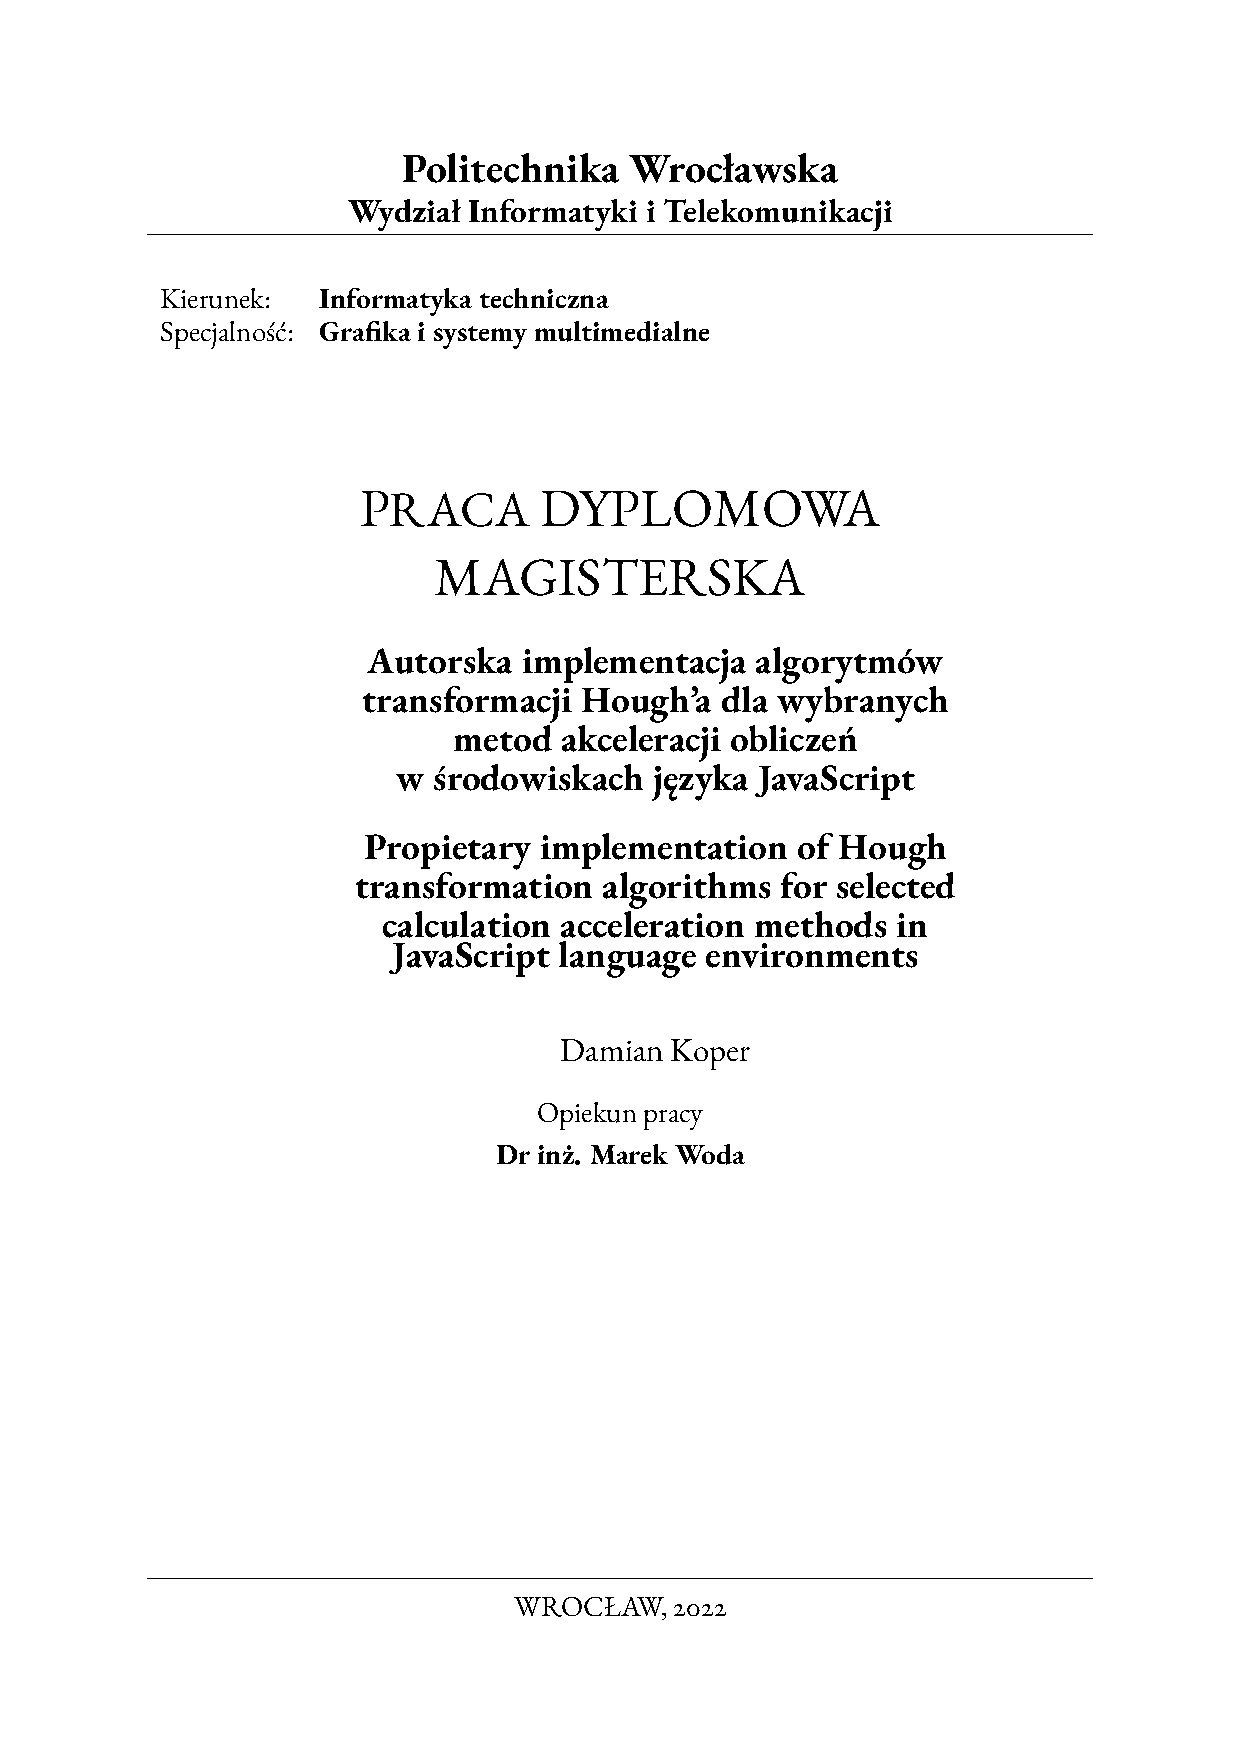
\includepdf[pages={1}]{../out/title}

\cleardoublepage
\thispagestyle{empty}
\begin{abstract}
   blabla
\end{abstract}
\mykeywords{raz, dwa, trzy, cztery}

{
    \selectlanguage{english}
    \begin{abstract}
        blabla in english
    \end{abstract}
    \mykeywords{one, two, three, four}
}
 
\pagestyle{outer}
\clearpage

\chapterstyle{noNumbered}  % Below there are declarations of various lists. Please comment out those which are too short (the list should contain at least 5 items)
\pagestyle{outer}
\mbox{}\pdfbookmark[0]{Table of contents}{spisTresci.1}
\tableofcontents*

\newpage
\mbox{}\pdfbookmark[0]{List of figures}{spisRysunkow.1}
%\addcontentsline{toc}{chapter}{Spis rysunków}
\listoffigures*

\newpage
\mbox{}\pdfbookmark[0]{List of tables}{spisTabel.1}
%\addcontentsline{toc}{chapter}{Spis tabel}
\listoftables*

\newpage
\mbox{}\pdfbookmark[0]{Spis listingów}{spisListingow.1}
%\addcontentsline{toc}{chapter}{Spis listingów}
\lstlistoflistings*

% Below there are inclusions of latex files
\chapter*{Skróty}\mbox{}\pdfbookmark[0]{Skróty}{skroty.1}
\label{sec:skroty}
\noindent
\begin{description}[labelwidth=*]
  \item [IDE] (ang.\ \emph{Integrated Development Environment})
  \item [API] (ang.\ \emph{Application Programming Interface})
  \item [CPU] (ang.\ \emph{Central Processing Unit})
  \item [GPU] (ang.\ \emph{Graphics Processing Unit})
  \item [GPGPU] (ang.\ \emph{General-purpose computing on graphics processing units})
  \item [ESSL] (ang.\ \emph{OpenGL ES Shading Language})
  \item [SPA] (ang.\ \emph{Single Page Application})
  \item [DOM] (ang.\ \emph{Document Object Model})
  \item [URL] (ang.\ \emph{Uniform Resource Locator})
  \item [NPM] (ang.\ \emph{Node Package Manager})
  \item [UMD] (ang.\ \emph{Universal Module Definition})
  \item [AMD] (ang.\ \emph{Asynchronous Module Definition})
  \item [ESM] (ang.\ \emph{ESModules, ECMAScript Modules})
  \item [LUT] (ang.\ \emph{Lookup Table})
  \item [PTLM] (ang.\ \emph{Point-to-line mapping})
  \item [LUT] (ang.\ \emph{Lookup Table})
  \item [SHT] (ang.\ \emph{Standard Hough Transform})
  \item [CHT] (ang.\ \emph{Circle Hough Transform})
  \item [WASM] (ang.\ \emph{WebAssembly})
  \item [SIMD] (ang.\ \emph{Single Input Multiple Data})
\end{description}
 % If abbreviations list is short, you can comment it out
\chapterstyle{default}{
\chapter{Wstęp}

Prawo Moore'a mówi, że liczba tranzystorów w~układach scalonych podwaja się co około dwa lata. Prawo Koomey'a opisuje natomiast trend wzrostu liczby obliczeń na jeden dżul energii, która podwaja się co 1.57 lat. Choć w~ostatnich latach, w~związku ze zmniejszającym się tempem miniaturyzacji tranzystorów, wartości te przestały być aktualne to wciąż mamy do czynienia ze zjawiskiem ustawicznego wzrostu mocy obliczeniowej. Dodatkowo, zgodnie z~obserwacją nazwaną prawem Huang'a - prezesa firmy NVIDIA, wzrost wydajności układów graficznych wzrasta więcej niż dwukrotnie co dwa lata\cite{tongo}, co świadczy o~obecnym rozwoju możliwości optymalizacji architektur i~programów wykorzystujących przetwarzanie masowo równoległe.  Wzrost wydajności z~kolei zwiększa możliwości wykorzystania algorytmów, które wcześniej były zbyt intensywne obliczeniowo i~nie mogły być wykorzystane w~rozwiązaniach produkcyjnych. Powszechnie dostępne wydajne maszyny dają również możliwości szybszego prototypowania rozwiązań większej liczbie osób, co z~kolei wpływa na rozwój samych algorytmów i~ich zastosowań. Algorytmy i~obliczenia opierają się na osiągnięciach analizy numerycznej oraz matematyki dyskretnej.

Analiza numeryczna zajmuje się opisywaniem i~analizą metod pozyskiwania wyników dla problemów matematycznych. Dzięki jej osiągnięciom możliwe jest budowanie algorytmów, które są kompletnym i~jednoznacznym opisem metody konstruowania rozwiązania owych problemów. Konstruowane algorytmy mogą mieć różne poziomy skomplikowania zaczynając od obliczania wartości funkcji, wielomianów, czy też znajdować rozwiązania układów równań. Dzięki nim możemy aproksymować wartości funkcji - obliczać pochodne oraz całki korzystając z~metod prostokątów, trapezów, czy Simpson'a. Możemy obliczać przybliżenia funkcji trygonometrycznych korzystając z~szeregów Taylor'a. Dzięki obliczeniom opartym o~algebrę liniową i~rachunek różniczkowy mogły rozwinąć się pola związana z~uczeniem maszynowym. Znajdowanie wektorów i~wartości własnych macierzy w~metodzie PCA w~celu redukcji wymiarowości danych, a~w końcu algorytmy propagacji wstecznej szczególnie wykorzystywane w~intensywnie rozwijającym się obszarze uczenia głębokiego\cite{phillips1996theory}.

Niezależnie od skali zaawansowania algorytmów dążą one do stanowienia rozwiązania konkretnych problemów świata rzeczywistego. Przykładem ich zastosowania jest przewidywanie pogody w~oparciu o~modele meteorologiczne, które zaczęło intensywnie rozwijać się wraz z~dostępem do coraz większej mocy obliczeniowej i~udoskonalaniem samych modeli. W~ciągu 15 lat, od 1971 roku, spełnialność prognoz 36-godzinnych zrównała się ze spełnialnością prognoz 72-godzinnych\cite{lynch2008origins}. Kolejnym wartym przytoczenia przykładem jest obszar analizy obrazów z~wyszczególnieniem zagadnienia ich klasyfikacji, gdzie wzrost mocy obliczeniowej pozwolił na rozwój algorytmów. W~ciągu 8 lat metryka dokładności klasyfikacji obrazów na zbiorze danych ImageNet wzrosła z~63\% do 90\%\cite{lynch2008origins,dai2021coatnet}.

Dynamiczny rozwój algorytmów napędzany jest przede wszystkim przez poszerzanie i~budowanie wiedzy domenowej, specyficznej dla rozwiązywanego problemu. Jednak, aby uczynić taki rozwój możliwym, musi być on oparty na niezbędnych filarach jakimi są oprogramowanie, które służy do prototypowania, a~następnie wdrażania rozwiązań oraz środowisko sprzętowe, które umożliwia przeprowadzanie obliczeń, wielokrotnych testów, prototypów na małą oraz wdrożeń na dużą skalę. Wraz ze wzrostem złożoności problemu liczba obliczeń niezbędnych do jego rozwiązania również rośnie i~w przypadku ich większości ten wzrost jest wykładniczy lub większy. Niezbędnym zatem jest, aby oprogramowanie potrafiło wykorzystać wszelkie dostępne metody akceleracji zarówno te związane z~optymalizacją samego algorytmu, jak i~te związane z~mechanizmami akceleracji sprzętowej.

\section{Istota rzeczy}

Wykonywanie obliczeń numerycznych wśród obecnie popularnych rozwiązań można podzielić na dwie grupy. Pierwsza z~nich używa specjalnie do tego celu stworzonego języka programowania, często również w~połączeniu ze zintegrowanym środowiskiem programistycznym (Integrated Development Environment, ang. IDE). Przykładem takiego rozwiązania jest środowisko i~język MATLAB\cite{matlab} oraz R\cite{r}, czy też środowisko Mathematica z~językiem Wolfram\cite{mathematica}.

Druga grupa używa języka ogólnego przeznaczenia do wykonywania obliczeń w~oparciu o~zewnętrzne biblioteki w~zdecydowanej większości udostępniane jako oprogramowanie open-source, które dostarczają wymagany zestaw funkcjonalności niwelując potrzebę ich ręcznej implementacji. Języki takie możemy podzielić na te niskiego poziomu, zapewniające wysoką wydajność, oraz te wysokiego poziomu, interpretowane, zapewniające większą wygodę użytkowania. Najbardziej popularnym tego typu środowiskiem jest język Python, którego społeczność stworzyła liczne biblioteki (w postaci pakietów) do przetwarzania danych, obliczeń numerycznych i~statystycznych, analizy obrazów, czy uczenia maszynowego. Najpopularniejsze z~nich podane zostały w~tabeli \ref{tab:py-js}. W~nawiasach została ujęta liczba pobrań danego pakietu w~przeciągu ostatniego tygodnia na dzień 2022-04-27. Dla punktu odniesienia warto dodać, że w~przeciągu tego samego tygodnia, w~całym ekosystemie, pobrano łącznie 3.409.997.407 pakietów \cite{pypi-stats}.

Biblioteki takich języków, czego przykładem jest biblioteka OpenCV, często implementowane są w~językach kompilowanych bezpośrednio do kodu maszynowego takich jak C++ czy Rust udostępniając jednolity interfejs, którego metody, poprzez powiązania, wywoływać mogą języki skryptowe wysokiego poziomu, takie jak już wspomniany Python. Takie rozwiązania zapewnia możliwość zbudowania wersji biblioteki kompatybilnej z~wieloma środowiskami i~językami na podstawie jednego kodu bazowego, poddając adaptacji tylko elementy architektury integrującej bibliotekę niskopoziomową i~język wysokiego poziomu. Skompilowana biblioteka poddana może być również procesom optymalizacji, co zwiększyć może jej wydajność. Wadę takiego rozwiązania stanowi konieczność kompilowania biblioteki niskiego poziomu dla wielu systemów operacyjnych, czy architektur procesora. Taka kompilacja odbywać może się przed publikacją samej biblioteki, a~gotowe artefakty pobierane są przez użytkownika w~momencie instalacji. Kompilacja może odbywać się również bezpośrednio na maszynie użytkownika w~momencie instalacji.

% TODO: diagram abstrakcji  codebase - binding - js/python/etc

Opisany podział nie skłania do uznania przewagi jednej z~grup nad drugą w~żadnym z~aspektów. W~środowiskach specyficznych i~zintegrowanych brakujące funkcjonalności mogą zostać dodane przez twórców jako biblioteki standardowe języka oraz zaimplementowane przez społeczność w~bibliotekach języków ogólnego przeznaczenia. Obie grupy rozwiązań z~reguły są w~stanie działać w~środowisku tego samego systemu operacyjnego i~wchodzić w~interakcje z~tym samym sprzętem, i~wykorzystać idące za tym możliwości akceleracji obliczeń. Jednak nie wszystkie języki ogólnego przeznaczenia i~technologie zyskały jednakową popularność w~obszarze obliczeń numerycznych mimo swojej ogólnej popularności. Przykładem takowych są technologie webowe z~językiem JavaScript na czele.

\subsection{Duża i~rosnąca rola technologii webowych}

Technologie webowe zdefiniować można jako narzędzia i~techniki umożliwiające wymianę danych pomiędzy różnymi urządzeniami przez internet. Technologie webowe mogą występować i~spełniać różne zadania na wielu poziomach architektury aplikacji. W~przypadku architektury klient-serwer środowiskiem frontend'owym umożliwiającym wyświetlanie i~obsługę graficznego interfejsu użytkownika zwykle jest przeglądarka internetowa, gdzie za jego implementację na najniższym poziomie abstrakcji odpowiadają języki HTML, CSS i~JavaScript. Serwerem może być na przykład aplikacja komunikująca się z~klientem za pomocą API zaimplementowanego w~architekturze REST, czy też za pomocą języka zapytań GraphQL uruchamiana w~środowisku NodeJS. 

Warto zaznaczyć, że serwer, jak i~klient, nie muszą być zaimplementowane z~wykorzystaniem języka JavaScript by być uznawanym jako aplikacja webowa. Języki takie jak PHP, Python, Ruby, Java, czy C\# także oferują zaawansowane frameworki, jednak to język JavaScript, ze względu na historię swojego rozwoju ściśle powiązaną z~przeglądarką internetową, uważany jest jako główne narzędzie i~czynnik rozwoju technologii webowych zarówno w~części klienckiej jak i~serwerowej. Potwierdzają to badania, gdzie JavaScript w~2021 roku dziewiąty rok z~rzędu został wyłoniony jako najpopularniejsza technologia wśród developerów \cite{stack2021}.

\begin{table}
    \caption{Popularne biblioteki do przetwarzania danych w~języku Python i~ich odpowiedniki w~języku JavaScript. Dane pochodzą z~serwisów kolejno PyPI Stats oraz NPM, a~w~nawiasach znajduje się tygodniowa liczba pobrań biblioteki.}
    \centering
    \renewcommand\arraystretch{1.2}
    \begin{tabularx}{\linewidth}[t]{p{5cm} p{4.5cm} X}
        \bfseries{Python} & \bfseries{JavaScript} & \bfseries{Zastosowanie} \\ \hline
        numpy (26.067.844) & numjs (533) & Operacje na macierzach \\ \hline
        pandas (19.778.648) & danfojs (1.029) & Operacje na strukturach danych \\ \hline
        scipy (9.986.376) & simple-statistics (87.882) \newline fft.js (8.027) & Operacje związane z~analizą numeryczną, przetwarzanie sygnałów, algebra liniowa. \\ \hline
        scikit-learn (7.705.438) & ml (156) & Uczenie maszynowe \\ \hline
        matplotlib (6.457.099) \newline plotly (1.632.246) & plotly.js (149.542) \newline c3 (83.564) & Wizualizacja danych \\ \hline
        tensorflow (3.348.986) & @tensorflow/tfjs (91.233) & Sieci neuronowe \\ \hline
        opencv-python (1.236.711) & OpenCV.js (b.d \cite{cv2-js}) \newline jimp (1.479.783) \newline image-js (4.103)        & Operacja na obrazach, computer vision \\ \hline

    \end{tabularx}
    \label{tab:py-js}
\end{table}

\subsubsection{JavaScript w~obliczeniach numerycznych}

Pomimo swojej popularności, w~przeciwieństwie do języka Python, język JavaScript nie zyskał popularności wśród zadań obliczeń inżynierskich, naukowych, statystycznych, obróbki i~analizy obrazów. Jest on starszy od języka JavaScript i~w przeciwieństwie do niego od początku mógł pełnić zadanie narzędzia do implementacji algorytmów obliczeniowych, podczas gdy JavaScript ograniczony był jedynie do jednowątkowego środowiska przeglądarki internetowej. Dopiero w~2009 roku, wraz z~pojawieniem się środowiska NodeJS, możliwe stało się uruchamianie kodu JavaScript po stronie serwera. Umożliwia to również powstały w~2018 roku środowisko Deno. 

Innym czynnikiem, który warunkuje tempo rozwoju i~potencjalny przepływ użytkowników ku lepszym ich zdaniem środowiskom jest dostępność metod akceleracji obliczeń, która warunkuje możliwości poprawy wydajności. W~konsekwencji przekłada się to na wygodę użytkowania i~możliwości prototypowania bardziej złożonych algorytmów dla problemów o~większych rozmiarach. Przykładem takich są algorytmy uczenia maszynowego, w~szczególności uczenia głębokiego.

Ostatnim z~analizowanych czynników jest architektura systemu pakietów, która jest ściśle powiązana ze środowiskami uruchomieniowymi, które z~nich korzystają. Pobierane pakiety zawierają biblioteki, które importowane są do projektu w~postaci modułów. Python posiada jeden format modułów w~przeciwieństwie do języka JavaScript ze względu na heterogeniczność środowisk jego wykonywania. Przeglądarka internetowa, NodeJS i~Dino mimo, że wykonują kod w~tym samym języku, posiadają znaczące różnice w~sposobie komunikacji z~użytkownikiem, systemem operacyjnym, w~dostępności metod akceleracji i~zarządzaniu modułami. Rodzi to problemy 

Obecnie jednak, z~technicznego punktu widzenia, nie istnieją zasadnicze różnice pomiędzy środowiskami języków Python i~JavaScript, które hamowałyby w~znacznym stopniu rozwój bibliotek służącym do prototypowania i~wdrażania aplikacji zajmującymi się obliczeniami numerycznymi w~środowiskach języka JavaScript.

W tabeli \ref{tab:py-js} przedstawiono porównanie popularnych bibliotek stosowanych przy obliczeniach numerycznych języka Python z~ich odpowiednikami w~języku JavaScript. Widać wyraźnie dysproporcję w~liczbie pobrań bibliotek pomiędzy językami. W~wielu przypadkach autorowi nie udało się znaleźć dokładnego odpowiednika danej biblioteki, a~znalezione zestawy bibliotek języka JavaScript nie pokrywają w~całości funkcjonalności biblioteki języka Python.

% https://github.com/iodide-project/awesome-browser-data-science-libraries#mathstatistics
% https://stackoverflow.com/questions/31412537/numpy-like-package-for-node

\section{Cel badań i~zawartość pracy}

\begin{wraptable}{r}{7.5cm}
    \vspace{-0.5cm}
    \begin{threeparttable}
        \caption{Analyzed acceleration methods and environments.}
        \label{tab:implemented}
        \setlength{\tabcolsep}{0.3em}
        \begin{tabularx}{7.5cm}{lllll }%
            \hline
                         & Chrome                            & Firefox                           & Node                              & Deno                              \\
            \hline
            Sequential   & \textcolor{blue}{\cmark}          & \textcolor{blue}{\cmark}          & \textcolor{blue}{\cmark}          & \textcolor{blue}{\cmark}          \\
            Native addon & \textcolor{red}{\xmark} \tnote{1} & \textcolor{red}{\xmark} \tnote{1} & \textcolor{blue}{\cmark}          & \textcolor{red}{\xmark} \tnote{2} \\
            asm.js       & \textcolor{blue}{\cmark}          & \textcolor{blue}{\cmark}          & \textcolor{blue}{\cmark}          & \textcolor{red}{\xmark} \tnote{2} \\
            WASM         & \textcolor{blue}{\cmark}          & \textcolor{blue}{\cmark}          & \textcolor{blue}{\cmark}          & \textcolor{red}{\xmark} \tnote{2} \\
            WASM+SIMD    & \textcolor{blue}{\cmark}          & \textcolor{blue}{\cmark}          & \textcolor{blue}{\cmark}          & \textcolor{red}{\xmark} \tnote{2} \\
            Workers      & \textcolor{blue}{\cmark}          & \textcolor{blue}{\cmark}          & \textcolor{blue}{\cmark}          & \textcolor{blue}{\cmark}          \\
            WebGL        & \textcolor{blue}{\cmark}          & \textcolor{blue}{\cmark}          & \textcolor{red}{\xmark} \tnote{2} & \textcolor{red}{\xmark} \tnote{1} \\
            WebGPU       & \textcolor{red}{\xmark} \tnote{3} & \textcolor{red}{\xmark} \tnote{3} & \textcolor{red}{\xmark} \tnote{1} & \textcolor{red}{\xmark} \tnote{3} \\
            \hline
        \end{tabularx}

        \begin{tablenotes}\footnotesize
            \item [1] Not available in environment
            \item [2] Requires external package or non-C++ codebase
            \item [3] Unstable or under a flag
        \end{tablenotes}

        \vspace{-0.5cm}
    \end{threeparttable}
\end{wraptable}

 
Celem niniejszej pracy jest zbadanie przystosowania środowisk języka JavaScript do przeprowadzania obliczeń numerycznych oraz wykonywania złożonych algorytmów. Analizie poddano popularne środowiska - NodeJS, Deno i~przeglądarki internetowe Google Chrome i~Mozilla Firefox. Dla tych środowisk zbadano dostępne metody akceleracji obliczeń, gdzie pojęcie akceleracji rozumiane jest jako każda modyfikacja algorytmu wpływająca pozytywnie na jego wydajność. Tyczy się to optymalizacji wersji sekwencyjnej algorytmu bez zmiany jego złożoności, jak i~jego modyfikację do wersji zrównoleglonej. Metody akceleracji zaimplementowane dla badanych środowisk przedstawione zostały w~tabeli \ref{tab:implemented}. Zostaną one opisane dokładnie w~dalszej części pracy. Analiza zorientowana jest na algorytmy analizy obrazów.


Na to złożone zagadnienie trzeba spojrzeć z~wielu perspektyw. Autor pracy abstrahuje jednak od zagadnienia poprawy złożoności obliczeniowej samego algorytmu w~wersji sekwencyjnej, ponieważ rozważania takie wykraczają poza zakładaną w~pracy tematykę, która koncentruje się na środowiskach języku JavaScript i~możliwościach tych środowisk, jak i~samego języka.

\subsection{Perspektywa wydajności}

Pierwszą z~perspektyw jest wydajność algorytmu postrzegana przez pryzmat środowiska, w~którym jest on wykonywany oraz wykorzystywanych przez niego metod akceleracji. W~pracy zbadano wydajność zaimplementowanego algorytmu z~wykorzystaniem metod wymienionych w~tabeli~\ref{tab:implemented}, które szczegółowo omówione zostały w~rozdziale \ref{sec:acc-methods}.

\subsection{Perspektywa kompatybilności i~budowania bibliotek}

Innym punktem widzenia jest kompatybilność budowanych bibliotek w~wielu środowiskach. Jednak każde z~nich jest na tyle zróżnicowane, że zbudowanie jednej wersji kodu źródłowego kompatybilnego z~nimi wszystkimi naraz jest wymagające, a~niekiedy niemożliwe. Analiza tego zagadnienia, możliwości i~ograniczeń modularności kodu języka JavaScript, dodatkowo w~aspekcie wykorzystywanych metod akceleracji, opisana została w~rozdziale \ref{sec:env-modules}.

\subsection{Perspektywa wygody użytkowania}

Celem autorów bibliotek jest dostarczenie rozwiązań, które przede wszystkim będą aktywnie wykorzystywane. Autor, razem z~opisem implementacji algorytmów i~ich późniejszego wykorzystania, w~rozdziale \ref{sec:implementation} analizuje możliwości i~sposoby interakcji ze środowiskami, wyświetlanie wyników, ładowanie danych oraz wewnętrzne mechanizmy przetwarzania danych związane również z~modelem wykonania języka JavaScript.

\subsection{Transformacja Hough'a jako wspólny mianownik analizy}

W celu porównania wydajności pomiędzy środowiskami dla tej samej metody akceleracji oraz porównania ich w~ramach jednego środowiska zaimplementowano algorytmy transformacji Hough'a (czyt. Haf'a), która dokładniej opisana został w~rozdziale \ref{sec:hough}. Jest to rodzina algorytmów deterministycznych wykorzystywana do detekcji kształtów parametrycznych i~nieparametrycznych na obrazach.  Własna implementacja algorytmów z~tej rodziny, w~przeciwieństwie do zestawów testowych takich jak na przykład Ostrich\cite{ostrich}, daje możliwości granularnej kontroli nad samą implementacją i~możliwości dostosowania jej do wszystkich analizowanych środowisk i~metod akceleracji. Samo wykrywanie kształtów na podstawie transformacji Hough'a jest intensywne obliczeniowo, wieloetapowe, wykorzystuje operacje zmiennoprzecinkowe, w~tym funkcje trygonometryczne, oraz zakłada wykonanie wielu iteracji po dużych, zależnych od rozmiaru problemu i~próbkowania, strukturach danych. Czynniki te czynią tę rodzinę algorytmów, zdaniem autora, dobrym punktem zaczepienia podczas szerokiej analizy środowisk i~metod akceleracji, które one udostępniają, co pozwala uzyskać ogólną orientację w~analizowanych perspektywach oraz wskazać wartościowe kierunki przyszłych badań. 

\subsection{Zawartość pracy}

Rozdział drugi opisuje język JavaScript, wprowadza w~zagadnienie jego modelu wykonania, środowisk oraz opisuje dostępne dla nich metody akceleracji i~sposoby budowania bibliotek. Wspólny mianownik analizy, czyli algorytmy transformacji Hough'a i~sposób ich działania opisany został w~rozdziale trzecim. Rozdział czwarty opisuje metodykę przeprowadzanych testów wydajności, dla potrzeb których zaimplementowana została osobna biblioteka odpowiedzialna za pomiary czasu wykonania, mając na uwadze jej kompatybilność ze wszystkimi środowiskami. Implementację algorytmów i~konsekwencje idące za stosowaniem poszczególnych rozwiązań opisuje rozdział piąty. Rozdział szósty przedstawia rezultaty testów wydajności ze wskazaniem na porównanie środowisk i~metod do bazowych wariantów sekwencyjnego wykonania algorytmu, a~rozdział siódmy stanowi podsumowanie całości rozważań i~eksperymentów oraz wskazuje zidentyfikowane problemy i~proponowane kierunki przyszłych badań.

\chapter{Język JavaScript}

JavaScript od momentu swojego powstania w~1995 roku stanowi jeden z~filarów rozwoju technologii webowych, zaczynając od dodania prostych mechanizmów interaktywności do statycznych stron internetowym, a~kończąc na byciu nieraz jedynym samodzielnym budulcem pełnowymiarowych aplikacji działających po stronie klienta i~serwera, aplikacji działających w~środowisku przeglądarki internetowej, ale też w~środowiskach natywnych, desktopowych i~mobilnych. Dlatego, aby zrozumieć w~pełni specyfikę problemu, który stanowi przystosowanie języka do wykonywania obliczeń numerycznych, w~tym rozdziale przybliżone zostały zagadnienia związane z~modelem wykonania, środowiskami oraz sposobami na podział kodu na moduły i~późniejsze ich wykorzystanie. Na końcu opisane zostały metody akceleracji, dla których przeprowadzono badania.



\section{Model wykonania}

Model wykonania języka JavaScript skoncentrowany jest w~głównej mierze na obsłudze zdarzeń. W~przeglądarce internetowej zdarzeniami takimi mogą być interakcje z~użytkownikiem, na przykład kiedy naciśnięty zostanie przycisk, albo interakcje z~siecią, kiedy otrzymamy odpowiedź na zapytanie z~wykorzystaniem obiektu \lstinline{XMLHttpRequest} lub skorzystamy z~Fetch API. Po stronie serwera zdarzeniami takimi mogą być odebranie zapytania, które serwer musi obsłużyć, obsługa strumieni, ale także wszelkie odpowiedzi na interakcje z~systemem operacyjnym. Podstawowymi interakcjami mogą być obsługa sygnałów, dostęp do plików, czy też obsługa sieci, która umożliwia połączenie na przykład z~bazą danych.

Zdarzenia te obsługuje pętla zdarzeń (ang. event loop). Na rysunku \ref{fig:event-loop} pokazano jej uproszczony model. Wyróżnia ona zadania, zwane także makro zadaniami, oraz mikro zadania. Dla każdego typu zadań utworzona zostaje osobna kolejka. Jeśli aktualnie wykonywane przetwarzanie sekwencyjne, którego ramki wywołań śledzone są na stosie, zakończy się, wtedy z~pętli zdarzeń pobierane i~wykonywane jest makro lub mikro zadanie. W~pierwszej kolejności wykonywane są wszystkie mikro zadania, a~gdy ich kolejka jest pusta, wykonywane jest kolejne makro zadanie.

Makro zadania dodawane są do kolejki, aby obsłużyć wspomniane już zdarzenia związane z~działaniami użytkownika lub inne zewnętrzne zdarzenia. Są one również dodawane do kolejki, kiedy mija czas zadany podczas wywołań funkcji \lstinline{setTimeout()} oraz \lstinline{setInterval()}. Warto zaznaczyć, że wywołania tych funkcji nie gwarantują wykonania dokładnie po zadanym czasie, ale traktują go jako próg czasowy, po jakim zadana funkcja zostanie dodana do kolejki makro zadań \cite{setTimeout}. Makro zadania dodane podczas jednej iteracji pętli nigdy nie zostaną wykonane w~tej samej iteracji.

Mikro zadania pochodzą tylko i~wyłącznie z~kodu użytkownika, bądź bibliotek i~wykorzystywane są do obsługi asynchronicznych zadań, zarządzania ich kolejnością i~obsługą błędów\cite{runtime}. Do ich tworzenia wykorzystuje się głównie obiekt \lstinline{Promise}, który reprezentuje zadanie, które w~przyszłości zakończy się pomyślnie lub błędem. Dla takiego obiektu zdefiniować możemy funkcje, które wykonają się podczas scenariusza pomyślnego (\lstinline{then}), błędnego (\lstinline{catch}) oraz zawsze (\lstinline{finally}) \cite{promise}. Mikro zadania pochodzić mogą również od obserwatorów na przykład \lstinline{MutationObserver}, czy \lstinline{ResizeObserver}.

Zrozumienie sposobu wykonywania kodu w~asynchronicznym modelu języka JavaScript jest kluczowe do efektywnego wykorzystania możliwości, jakie idą za metodami akceleracji, których użycie możliwe jest tylko i~wyłącznie poprzez asynchroniczne wywołania. Opisane w~sekcji \ref{sec:acc-methods} metody bazujące na Worker'ach oraz WebGL wymagają interakcji poprzez wywołania asynchroniczne. Na listingu \ref{lst:async} pokazano przykład kodu asynchronicznego. Wywołania \mbox{\lstinline{console.log}} wykonają się, zawsze drukując liczby w~kolejności od 1 do 6.

\lstinputlisting[language=JavaScript, caption=Przykład kodu demonstrujący mechanizmy asynchroniczności w~języku JavaScript., label=lst:async] {./code/async.js}

Linijki 1 oraz 6 zostają wykonane synchronicznie. \lstinline{Promise} w~linijce 5 zostaje wykonany jako następny, ponieważ jako mikro zadanie, wykona się zaraz po operacjach synchronicznych. Następnie funkcje \lstinline{setTimeout} wykonają się w~kolejności ich wywołania, gdzie w~linijkach 2-4 na ich kolejność wpływ maja mechanizm \lstinline{Promise}. Timeout z~linijki 3, a~potem 4 zostają wywołane jaki pierwsze. Jako ostatni wykonuje się timeout z~linijki 2, ponieważ jego wywołanie, w~postaci mikro taska, przeniesione zostało na koniec wykonania synchronicznego.

\begin{figure}
    \centering
    

\begin{tikzpicture}

\node[label=below:Event Loop,minimum size=1.9cm] (loop) at (0,-8) {\scalefont{4}$\circlearrowleft$};

% \node[rectangle, draw, minimum width=3cm, minimum height=8cm, anchor=north] (Heap_frame) at (0,0) {};
% \node[minimum width=3cm, below=0.25 of Heap_frame.north] (Heap)  {Heap} ;
% \node[rectangle, draw, minimum width=1cm, minimum height=1cm, below right=0.54 and 0.33 of Heap.west] (A) {\lstinline{a}} ;
% \node[rectangle, draw, minimum width=1cm, minimum height=1cm, right=0.33 of A] (B)  {\lstinline{b}} ;
% \node[rectangle, draw, minimum width=1cm, minimum height=1cm, below=0.33 of B] (C)  {\lstinline{c}} ;
% \node[rectangle, draw, minimum width=1cm, minimum height=1cm, left=0.33 of C] (D)  {\lstinline{d}} ;
% \node[rectangle, draw, minimum width=1cm, minimum height=1cm, below=0.33 of D] (E)  {\lstinline{e}} ;
% \node[rectangle, draw, minimum width=1cm, minimum height=1cm, right=0.33 of E] (F)  {\lstinline{f}} ;
% \node[rectangle, draw, minimum width=1cm, minimum height=1cm, below=0.33 of E] (G)  {\lstinline{f}} ;

\node[rectangle, draw, minimum width=3.5cm, minimum height=6cm, anchor=north] (Stack_frame) at (0,0) {};
\node[minimum width=3cm, minimum height=1cm, below=0 of Stack_frame.north] (Stack)  {Stack} ;
\node[rectangle, draw, minimum width=3cm, minimum height=0.6cm, below=0 of Stack] (exec) {\lstinline{exec()}} ;
\node[rectangle, draw, minimum width=3cm, minimum height=0.6cm, below=0 of exec] (A) {\lstinline{function A()}} ;
\node[rectangle, draw, minimum width=3cm, minimum height=0.6cm, below=0 of A] (B)  {\lstinline{function B()}} ;
\node[rectangle, draw, minimum width=3cm, minimum height=0.6cm, below=0 of B] (C)  {\lstinline{function C()}} ;
\node[rectangle, draw, minimum width=3cm, minimum height=0.6cm, below=0 of C] (D)  {\lstinline{function D()}} ;
\node[rectangle, draw, minimum width=3cm, minimum height=0.6cm, below=0 of D] (E)  {\lstinline{function E()}} ;

% \path[->,thick] (1.5,-7) edge (2,-7);
% \path[<-,thick] (1.5,-7.5) edge (2,-7.5);


\node[rectangle, draw, minimum width=4.5cm, minimum height=5.2cm, anchor=north] (APIs_frame) at (11.5,0) {};
\node[minimum width=3cm, minimum height=1cm,, below=0 of APIs_frame.north] (APIs)  {APIs} ;
\node[rectangle, draw, minimum width=4cm, minimum height=0.75cm, below=0 of APIs] (main) {Fetch API} ;
\node[rectangle, draw, minimum width=4cm, minimum height=0.75cm, below=0 of main] (A) {Image Capture API} ;
\node[rectangle, draw, minimum width=4cm, minimum height=0.75cm, below=0 of A] (B)  {WebSocket API} ;
\node[rectangle, draw, minimum width=4cm, minimum height=0.75cm, below=0 of B] (C)  {Clipboard API} ;
\node[rectangle, draw, minimum width=4cm, minimum height=0.75cm, below=0 of C] (D)  {...} ;

\node[rectangle, draw, minimum width=11cm, minimum height=1cm, anchor=north east] (macro_frame) at (13.75,-6) {};
\node[ anchor=south east, above left=0 of macro_frame, anchor=south west] {Macro-task queue};

\node[rectangle, draw, minimum height=0.6cm, right=0.2 of macro_frame.west] (macroA)  
    {\lstinline{setTimeout()}} ;
\node[rectangle, draw, minimum height=0.6cm, right=0.2 of macroA] (macroB)  
    {\lstinline{setInterval()}} ;
\node[rectangle, draw, minimum height=0.6cm, right=0.2 of macroB] (macroC)  
    {\lstinline{fetch()}} ;
\node[rectangle, draw, minimum height=0.6cm, right=0.2 of macroC] (macroD)  
    {\lstinline{...}} ;

\node[rectangle, draw, minimum width=11cm, minimum height=1cm,  anchor=north east, below right=1.5cm and 0cm of macro_frame.west] (micro_frame)  {};
\node[ anchor=south east, above left=0 of micro_frame, anchor=south west] {Micro-task queue};

\node[rectangle, draw, minimum height=0.6cm, right=0.2 of micro_frame.west] (microA)  
    {\lstinline{Promise.then()}} ;
\node[rectangle, draw, minimum height=0.6cm, right=0.2 of microA] (microB)  
    {\lstinline{queueMicrotask()}} ;
\node[rectangle, draw, minimum height=0.6cm, right=0.2 of microB] (microC)  
    {\lstinline{...}} ;

\path [ultra thick,latex-] (loop) edge (macro_frame.west);
\path [ultra thick,latex-] (loop) edge (micro_frame.west);
\path [ultra thick,-latex] (loop.north) edge (Stack_frame);

\draw [ultra thick,-latex] (APIs_frame.south) -- (APIs_frame|-macro_frame.north);
\draw [ultra thick,-latex] (Stack_frame) -- (APIs_frame.west|-Stack_frame);


\end{tikzpicture}

    \caption{Uproszczony model pętli zdarzeń środowisk języka JavaScript w~wariancie z~wyróżnieniem API przeglądarek internetowych.}
    \label{fig:event-loop}
\end{figure}

\section{Środowiska JavaScript}
\label{sec:env-modules}

Rosnąca popularność języka JavaScript i~idących za jego stosowaniem możliwości przyspieszyła rozwój środowisk, w~których kod języka mógł być wykonywany. Pierwszym z~nich była przeglądarka internetowa. 

\subsection{Przeglądarka internetowa}

Głównym zadaniem przeglądarki internetowej jest pobieranie z~sieci i~wyświetlanie zawartości użytkownikowi oraz obsługa jego interakcji. Najważniejszym komponentem przeglądarki jest silnik renderujący, który zawiera między innymi silniki odpowiedzialne za parsowanie i~renderowanie struktury modelu DOM, adaptery służące do wywołań dostępnych bibliotek graficznych (OpenGL, Vulcan, DirectX) oraz silnik JavaScript. Z~perspektywy problemu stawianego w~tej pracy to właśnie silnik JavaScript jest najważniejszym komponentem silnika renderującego. Silnik języka zajmuje się parsowaniem, kompilacją do bytecode'u, interpretowaniem oraz późniejszą optymalizacją kodu. Posiada wiele możliwości optymalizacji spekulatywnej z~racji na specyfikę języka, który jest dynamicznie typowany \cite{meurer_2017}.

Popularnymi silnikami renderującymi są Blink z~silnikiem JavaScript V8 \cite{V8} oraz Gecko z~silnikiem JavaScript SpiderMonkey \cite{spidermonkey}. Silniki JavaScript skupione są na szybkim i~efektywnym wykonywaniu kodu i~nie zajmują się asynchronicznością i~pętlą zdarzeń. Odpowiedzialne za to są równolegle biblioteki. W~przeglądarce Google Chrome pętlę zdarzeń implementuje biblioteka LibEvent \cite{libevent}.

\subsection{NodeJS}

NodeJS jest powstałym w~2009 roku środowiskiem, które było odpowiedzią na architekturę pozostałych rozwiązań serwerowych, które angażują wiele procesów i~wątków do obsługi wielu zapytań w~tym samym czasie. Rodzi to problemy związane z~koniecznością przełączania kontekstu pomiędzy procesami oraz większe zapotrzebowanie na pamięć. Również każda operacja wejścia-wyjścia musi być synchroniczna, co prowadzi do zablokowania całego procesu w~oczekiwaniu na odpowiedź \cite{nodejs}.

Problemy te rozwiązało środowisko NodeJS, napisane w~C++ i~oparte na silniku V8. Razem biblioteką LibUv \cite{libuv} implementującą pętlę zdarzeń w~ramach jednego procesu wykonującego kod JavaScript użytkownika oraz wielu wątków, które realizują oczekiwanie na operacje asynchroniczne, pozwoliło rozwiązać problem operacji wejścia-wyjścia pozwalając w~ramach tych samych zasobów sprzętowych osiągnąć lepsza wydajność niż popularny serwer Apache \cite{node-apache}. Na rysunku \ref{fig:nodejs} pokazano architekturę środowiska NodeJS, która stoi pomiędzy aplikacją, a~systemem operacyjnym.

\begin{figure}
    \centering
    

\begin{tikzpicture}

\node[fill=red!50, draw, rectangle, anchor=north west, minimum width=12cm, minimum height=0.75cm]  at (0,0.85) {Application};

\node[fill=green!50, draw, rectangle, anchor=north west, minimum width=12cm, minimum height=0.75cm] at (0,0) {NodeJS API};
\node[fill=blue!20, draw, rectangle, anchor=north west, minimum width=7.95cm, minimum height=0.75cm]  at (0,-0.85) {NodeJS Bindings};
\node[fill=blue!20, draw, rectangle, anchor=north west, minimum width=3.95cm, minimum height=0.75cm]  at (8.05,-0.85) {C/C++ Addons};
\node[fill=orange!50, draw, rectangle, anchor=north west, minimum width=1.9cm, minimum height=0.75cm] (A)  at (0,-1.7) {V8};
\node[fill=violet!50, draw, rectangle, anchor=north west, minimum width=1.9cm, minimum height=0.75cm, right=0.1 of A] (B) {LibUv};
\node[fill=blue!20, draw, rectangle, anchor=north west, minimum width=1.9cm, minimum height=0.75cm, right=0.1 of B] (C) {c-ares};
\node[fill=blue!20, draw, rectangle, anchor=north west, minimum width=1.9cm, minimum height=0.75cm, right=0.1 of C] (D) {llhttp};
\node[fill=blue!20, draw, rectangle, anchor=north west, minimum width=1.9cm, minimum height=0.75cm, right=0.1 of D] (E) {OpenSSL};
\node[fill=blue!20, draw, rectangle, anchor=north west, minimum width=1.9cm, minimum height=0.75cm, right=0.1 of E] (F) {zlib};

\node[fill=black!20, draw, rectangle, anchor=north west, minimum width=12cm, minimum height=0.75cm]  at (0,-2.55) {Operating system};

\end{tikzpicture}
 
    \caption{Model architektury środowiska NodeJS.}
    \label{fig:nodejs}
\end{figure}

\subsection{Deno}

Deno powstał w~2018 roku, a~jego wersja 1.0.0 wydana została w~2020 roku. Jest to środowisko aspirujące do bycia następcą NodeJS rozwiązując jego problemy związane z~bezpieczeństwem, systemem budowania zależności bibliotek, czy importowania zależności \cite{deno}. Podobnie jak NodeJS do wykonywania kodu JavaScript wykorzystuje silnik V8, ale napisany jest w~języku Rust. Do obsługi asynchroniczności i~pętli zdarzeń wykorzystuje bibliotekę Tokio \cite{tokio}. W~przeciwieństwie do NodeJS i~przeglądarek internetowych obsługuje natywnie TypeScript.

\section{Modularność i~kompatybilność kodu}

Kolejnym ważnym aspektem rozważań jest modularność i~kompatybilność kodu pomiędzy środowiskami. Rozwój bibliotek języków jest naturalnym krokiem ewolucji ich ekosystemów i~aby taki ekosystem był ogólnodostępny, biblioteki dostępne są dla wszystkich w~postaci scentralizowanego rejestru paczek. 

\subsection{Modularność}

Dla środowiska NodeJS najpopularniejszym rejestrem jest \textit{npm registry} (node package manager). Za pomocą narzędzia o~tej samej nazwie można instalować i~zatrzaskiwać wersję paczek, które trafiają do folderu \lstinline{node_modules}, w~którym środowisko NodeJS domyślnie poszukuje kodu podczas importu paczek. Zainstalowane paczki są opisane wraz z~ich wersją w~pliku \mbox{\lstinline{package.json}} i~\lstinline{package-lock.json}, gdzie pierwszy z~nich zawiera wymaganą wersję zapisaną w~konwencji Semver \cite{semver}, a~drugi zatrzaśnięte zainstalowane wersje, co pozwala odtworzyć dokładną strukturę zależności.

Przeglądarki internetowe z~kolei pobierają dodatkowe biblioteki poprzez umieszczenie tagów \lstinline{<script/>} w~dowolnym miejscu na stronie, często z~użyciem sieci CDN (ang. content delivery network). \textit{npm} jest również popularnym rozwiązaniem służącym do dostarczania modułów niezbędnych do funkcjonowania stronom internetowym, jednak odbywa się to pośrednio. Za pomocą narzędzi zwanych bundler'ami, ze wszystkich niezbędnych zależności - właściwego kodu strony oraz zewnętrznych bibliotek instalowanych przy pomocy narzędzia \textit{npm}, budowany jest pojedynczy plik, który następnie jest ładowany przez przeglądarkę. Pomaga to zaoszczędzić liczbę połączeń przeglądarki do serwerów, a~co za tym idzie zaoszczędzić czas spędzony na inicjowaniu połączenia i~pobieraniu danych w~szczególności, że liczba możliwych otwartych połączeń przez przeglądarkę internetową jest limitowana (10 w~Google Chrome). Często obecnie budowane są dwa lub więcej plików - jeden z~bibliotekami zewnętrznymi oraz jeden lub więcej z~właściwym kodem strony w~celu wykorzystania mechanizmów pamięci podręcznej przeglądarki oraz dynamicznego i~opóźnionego ładowania niezbędnego kodu, co przyspiesza ładowanie strony. Popularnymi bundler'ami są Webpack, Snowpack, Parcel, Rollup oraz Vite.

Deno próbuje rozwiązać problem importowania modułów w~NodeJS, który wynika z~scentralizowanego rejestru i~paczek oraz z~faktu istnienia plików \lstinline{package*.json} i~konieczności wykonania procesu instalacji. Pobiera on zależności bezpośrednio z~sieci i~umieszcza w~pamięci podręcznej. Link do zależności jest jej jednoznacznym identyfikatorem, a~to znaczy, że powinien zawierać wersję paczki i~nigdy nie zmienić swojej zawartości. Pobranie i~kompilacja zależności w~czasie wykonania programu likwiduje potrzebę przechowywania listy zależności i~ich wersji oraz niweluje potrzebę ich instalacji. Deno wykorzystuje opisany w~dalszej części rozdziału format modułów ESM.

Niezależnie od tego gdzie przetrzymywane są moduły oraz w~jaki sposób są zarządzane przez środowisko, muszą one być finalnie przez nie skonsumowane. Mogą być one użyte bezpośrednio, ale też przetransformowane w~procesie budowania biblioteki, która będzie potem dalej konsumowana, czy paczki dla przeglądarki internetowej. W~procesie ewolucji ekosystemu języka JavaScript wykształciło się wiele formatów modułów. Niektóre z~nich są kompatybilne tylko z~przeglądarką internetową, niektóre tylko ze środowiskiem NodeJS bądź Deno.  

\subsubsection{AMD}

AMD (Asynchronous Module Definition) jest sposobem ładowania zależności w~przeglądarkach internetowych. Rozwija wzorzec modułów JavaScript \cite{jsmodulepattern} poprzez dodanie asynchronicznego pobierania i~ładowania zależności. Moduł jest funkcją, dzięki czemu zadeklarowane zmienne nie wyciekają poza jej zakres, a~jej wartość zwracana stanowi wartość, którą taki moduł eksportuje. Zadeklarowanie modułu i~jego zależności w~formacie AMD umożliwia funkcja \lstinline{define}.

\subsubsection{CommonJS}

Format CommonJS utworzony został na potrzeby środowiska NodeJS i~jest tam do dzisiaj wykorzystywany. Używa on globalnie dostępnej funkcji \lstinline{require}, która jako argument przyjmuje nazwę modułu lub relatywną ścieżkę do pliku \lstinline{*.js}, jednak z~pominięciem jego rozszerzenia, co stanowi problem podczas wyszukiwania modułów przez środowisko. Moduł może eksportować funkcje i~wartości poprzez dodanie ich do obiektu \lstinline{module.exports}. Pliki z~modułami w~tym formacie, aby lepiej je identyfikować, mogą mieć rozszerzenie \lstinline{*.cjs}.

\subsubsection{UMD}

UMD (Universal Module Definition) nie stanowi samodzielnego formatu, ale integruje formaty AMD, CommonJS oraz użycie zmiennych globalnych do definicji modułu i~jego zależności. Wyewoluował on z~potrzeby tworzenia bibliotek kompatybilnych z~wieloma środowiskami, dla których nie trzeba budować wielu wersji w~różnych formatach.

\subsubsection{Moduły ECMAScript}

Brak kompatybilności i~wiele formatów modułów, gdzie każde środowisko zaproponowało swój własny, wymusiło ich standaryzację w~specyfikacji języka. ECMAScript, którego implementacją jest JavaScript, w~wersji 2015 (zwanej również ES6) wprowadza definicję modułów zwanych ESModules, ESM \cite{ESModules}. Obecnie wspierane są one przez wszystkie analizowane tutaj środowiska i~są zalecaną metodą importowania zależności. Używają one słów kluczowych \lstinline{import} oraz \lstinline{export} tak, jak zostało to pokazane na listingu \ref{lst:esm}. Od wersji ES11 specyfikacji możliwe stało się dynamiczne importowanie modułów podczas wykonania, gdzie jako rezultat otrzymujemy obiekt \mbox{\lstinline{Promise}}. Pliki z~modułami w~tym formacie, aby lepiej je identyfikować, mogą mieć rozszerzenie \mbox{\lstinline{*.mjs}}. Wszystkie biblioteki wykorzystujące metody akceleracji badane w~tej pracy budowane są z~wykorzystaniem ESM.

\begin{lstlisting}[language=JavaScript, caption=Przykład wykorzystania ECMAScript Modules, label=lst:esm]
// main.mjs
import { add } from "./module"
console.log(add(2+2));

// module.mjs
export function add(foo, bar) { return foo + bar; }
\end{lstlisting}

\subsection{Kompatybilność}

Szerokie starania w~standaryzacji modułów umożliwiają tworzenie kodu kompatybilnego z~wieloma środowiskami. Jeśli jednak kod ten korzysta z~funkcjonalności samego środowiska, która istnieje w~pozostałych środowiskach, ale ich API nie są ze sobą zgodne, problem kompatybilności między środowiskami wciąż występuje. Wprowadza to niechciane mechanizmy do kodu wykrywające środowisko i~wymusza wykorzystanie wzorców projektowych takich jak \textit{adapter}, w~celu obsługi wszystkich wariantów API.

Przykładem takiego rozwiązania jest biblioteka \textit{axios}, która służy do wykonywania zapytań HTTP. W~środowisku przeglądarki internetowej do wykonywania zapytań wykorzystuje obiekt \lstinline{XMLHttpRequest}, a~w środowisku NodeJS wbudowany moduł \textit{http}. Rozwiązaniem problemu w~tym przypadku może być użycie Fetch API, które jako pierwsze zadebiutowało w~przeglądarkach internetowych oraz zaadaptowane zostało przez NodeJS, a~w Deno jest ono domyślnie przewidzianą formą wykonywania zapytań HTTP.

Innym przykładem braku kompatybilności pomiędzy podobnymi funkcjonalnościami jest wielowątkowość, która istnieje pod abstrakcją Worker'ów i~dokładnie zostanie omówiona w~rozdziale \ref{sec:acc-methods}. Przeglądarki internetowe oraz Deno, który ma na celu możliwie zbliżyć się do nich ze swoim API, implementują Web Worker API. NodeJS z~kolei do obsługi Worker'ów wykorzystuje wbudowany moduł \textit{worker\_threads}, który różni się od jego odpowiedników w~pozostałych środowiskach.    

\section{Metody akceleracji}
\label{sec:acc-methods}

Akceleracja obliczeń jest niekończącą się pogonią za nieskończenie krótkim czasem wykonania algorytmów. Zdaniem autora powinna być ona brana pod uwagę na każdym etapie ich rozwoju - od etapu prototypowania, do wdrożeń produkcyjnych, ponieważ na każdym z~nich może przynieść wymierne korzyści. Wspomnianą w~poprzednim rozdziale akcelerację praca traktuje jako wszelkie metody przyspieszające wykonywanie algorytmu.

\subsection{Optymalizacja wykonania sekwencyjnego}

Pierwszym aspektem, na który trzeba zwrócić uwagę jest sama interakcja z~silnikiem języka i~wykorzystanie jego możliwości oraz tego, w~jaki sposób potrafi on optymalizować wykonywany kod. Poprzez kompilację kodu Just-In-Time (JIT), czyli bezpośrednio przed jego wykonaniem oraz możliwość powtarzania tego procesu wykorzystując heurystyki dla zebranych danych, możliwe jest przyspieszenie wykonania kodu \cite{meurer_2017}. W~przypadku silnika V8 kod najpierw trafia do interpretera o~nazwie Ignition, gdzie kompilowany jest do bytecode'u, który zamieniany jest na instrukcje zgodne z~architekturą procesora. Równolegle bytecode wysyłany jest do kompilatora TurboFan, gdzie przechodzi optymalizację na poziomie funkcji, w~przeciwieństwie do innych rozwiązań JIT, które identyfikują wielokrotnie wykonywaną część bytecode'u \cite{meurer_2019}. Optymalizacja ta jest ograniczona do funkcji o~maksymalnym rozmiarze bytecode'u równym 60KB, więc ważne jest, aby umiejętnie rozbijać kod algorytmu na funkcje i~moduły. W~przeszłości podjęto również próby wykorzystania spekulacyjnego zrównoleglania kodu po stronie silnika JavaScript (Thread-level Speculation). Przyniosło to dobre rezultaty, jednak ta metoda optymalizacji nie jest implementowana w~popularnych silnikach \cite{martinsen2017combining}.

Osoba projektująca dany algorytm może celowo unikać konstrukcji języka oraz niektórych wzorców, aby wspomóc mechanizmy optymalizacji i~zwiększyć wydajność w~skrajnych przypadkach nawet o~25\% (\cite{gong2015jitprof}, \cite{selakovic2016performance}). Dobrą praktyką jest stosowanie typowanych tablic (Typed Array) do przechowywania danych binarnych oraz danych o~znanym typie. Innym sposobem poprawny wydajności jest modyfikacja algorytmu tak, aby zredukować obciążenie związane z~obliczeniami zmiennoprzecinkowymi, na przykład poprzez stosowanie stablicowanych wartości funkcji trygonometrycznych (LUT).

\subsection{Natywne moduły}

Środowiska NodeJS i~Deno działające po stronie serwera pozwalają na uruchomienie z~ich poziomu bibliotek skompilowanych do kodu maszynowego konkretnej architektury. Deno pozwala uruchomić funkcję ze skompilowanego kodu języka Rust do postaci biblioteki na różnych platformach (\lstinline{*.so}, \lstinline{*.dll}, \lstinline{*.dylib}). NodeJS natomiast posiada własny system budowania natywnych modułów z~kodu C++ o~nazwie \textit{node-gyp}, którego zależnością jest język Python.

Zaletą korzystania z~natywnych modułów jest możliwość wykorzystania metod optymalizacji specyficznych dla platformy sprzętowej, jakie oferują języki niskiego poziomu kompilowane do kodu maszynowego. Metodę tę można rozwinąć o~metody akceleracji dostępne w~językach źródłowych, których przykładem może być wielowątkowość z~wykorzystaniem biblioteki \lstinline{pthreads}. Do wad takiego rozwiązania zaliczyć można konieczność pobierania lub budowania natywnych zależności w~momencie instalacji biblioteki oraz ogólną kompatybilność, która wykracza poza środowisko języka JavaScript. Wadą, która wpływa w~znaczącym stopniu na wydajność w~specyficznych przypadkach jest brak bezpośredniego dostępu do pamięci silnika JavaScript, co skutkuje koniecznością kopiowania danych w~warstwie powiązania natywnego modułu z~kodem języka JavaScript. Dla dużych danych proces ten okazać się może wąskim gardłem algorytmu.

\subsection{WebAssembly}

Kolejną metodą akceleracji wykonania sekwencyjnego jest WebAssembly (WASM), który jest językiem niskiego poziomu. Stanowi on cel kompilacji języków takich jak C++, czy Rust i~pozwala uruchamiać w~środowisku webowym złożone aplikacje, których wcześniejsze uruchomienie nie było możliwe ze względu na konieczność parsowania i~kompilacji dużej ilości kodu. Umożliwiło to na przykład łatwe przeniesienie aplikacji napisanych w~języku C++ z~wykorzystaniem biblioteki Qt i~uruchomienie ich w~przeglądarce internetowej \cite{qt-wasm}. Kolejnym przykładem jest jeden z~backend'ów biblioteki Tensorflow.js \cite{tensorflowjs}, która umożliwia trenowanie i~wdrażanie modeli uczenia maszynowego. Dzięki bibliotece PyScript, która portuje implementację języka Python napisaną w~C do języka WebAssembly, możliwe stało się wykonywanie kodu języka w~przeglądarce internetowej \cite{pyscript}.

\begin{lstlisting}[language=C++, caption=Funkcja licząca silnię w~języku C/C++, label=lst:factorial-cpp]
int factorial(int n) {
    if (n == 0)
        return 1;
    else
        return n * factorial(n-1);
}
\end{lstlisting}
    
\begin{lstlisting}[language=WASM, caption=Funkcja licząca silnię w~języku WASM, label=lst:factorial-wasm]
(func (param i64) (result i64)
    local.get 0
    i64.eqz
    if (result i64)
        i64.const 1
    else
        local.get 0
        local.get 0
        i64.const 1
        i64.sub
        call 0
        i64.mul
    end)
\end{lstlisting}

Wydajność kodu WebAssembly zbliżona jest do wykonania natywnego. Moduły operują na liniowym modelu danych, który nie jest współdzielony z~kodem języka JavaScript. Podobnie jak w~przypadku natywnych modułów występuje konieczność transformacji i~kopiowania danych do pamięci modułu, co może rodzić problemy z~wydajnością. Na listingu \ref{lst:factorial-cpp} przedstawiono funkcję liczącą silnię, która na listingu \ref{lst:factorial-wasm} została zapisana w~jej odpowiedniku w~WASM. WebAssembly przetwarzany jest w~postaci binarnej i~działa jak maszyna stosowa, a~na potrzeby analizy zapisywany jest w~formacie tekstowym w~postaci S-wyrażeń.

\subsubsection{asm.js}

Poprzednikiem WebAssembly był asm.js - podzbiór języka JavaScript w~procesie kompilacji z~języków źródłowych zoptymalizowany pod kątem wydajności wykonania i~specjalnie interpretowany przez przeglądarki wykorzystując kompilację Ahead-Of-Time. Kompilację tę wspiera do dziś jedynie przeglądarka Firefox, jednak optymalizacje silnika V8 Google Chrome 28 zapewniły dwukrotny wzrost wydajności podczas wykonania asm.js \cite{asm.js-chrome}. Nie jest on już rozwijany i~został wyparty przez WebAssembly.

\subsubsection{SIMD}

WebAssembly jest w~stanie wykorzystać architekturę SIMD (Single Instruction, Multiple Data), używając rejestrów i~instrukcji wektorowych \cite{wasm-simd}. Kompilatory takie jak LLVM potrafią, w~procesie auto-wektoryzacji wykorzystać instrukcje wektorowe, aby przyspieszyć działanie pętli oraz połączyć inne masowe operacje logiczne i~arytmetyczne. Wektoryzację taką można również przeprowadzić ręcznie wykorzystując funkcje, które operują bezpośrednio na typach wektorowych.

\subsection{Współbieżność}

W środowisku przeglądarki internetowej współbieżność osiągnięta może być tylko na poziomie wielu wątków, poprzez zastosowanie Worker'ów. Każdy Worker funkcjonuje jako osobny wątek w~ramach tego jednego procesu. Posiada on własną pętlę zdarzeń i~z głównym wątkiem komunikuje się jedynie asynchronicznymi wiadomościami. Poza obiektem \lstinline{SharedArrayBuffer}, wspieranego przez interfejs operacji atomowych \lstinline{Atomic}, aby zapobiec problemowi wyścigów, Worker'y nie współdzielą pamięci. Dane w~wiadomościach przekazywane są z~użyciem algorytmu klonowania strukturalnego, który wspiera natywne typy takie jak tablice, mapy, czy sety \cite{structured-clone}. Nie możliwe jest natomiast kopiowanie funkcji zdefiniowanych przez użytkownika oraz węzłów drzewa DOM, ponieważ tylko wątek główny może być odpowiedzialny za renderowanie widoku strony. Aby uniknąć procesu klonowania dużych zmiennych, które chcemy przenieść do Worker'a, i~które nie są potrzebne nam w~wątku głównym, możemy użyć obiektów \lstinline{Transferrable}, które jeśli wskazane, zostają przeniesione do kontekstu Worker'a, a~nie skopiowane, oszczędzając w~ten sposób pamięć i~czas procesora.

W środowiskach działających po stronie serwera współbieżne wykonanie możliwe jest przy zastosowaniu Worker'ów, ale również poprzez uruchomienie podprocesów, z~którymi można komunikować się poprzez standardowe strumienie wejścia oraz wyjścia, a~w przypadku NodeJS, również poprzez mechanizm wiadomości, który zajmuje się ich automatycznyą serializacją i~parsowaniem. 
 
\subsection{GPGPU}

GPGPU (ang. General-purpose computing on graphics processing units) zakłada użycie układów graficznych do wykonywania obliczeń ogólnego przeznaczenia, które do tej pory wykonywane były na CPU. W~środowiskach desktopowych, możemy wykorzystać takie układy używając rozwiązań powiązanych z~architekturą układu, czego przykładem jest NVIDIA CUDA. Możemy również skorzystać z~framework'ów implementujących warstwę abstrakcji będąc kompatybilnymi z~wieloma platformami i~architekturami jak na przykład OpenCL. 

Środowiska webowe zorientowane są na jak największą kompatybilność pomiędzy platformami, a~pierwotnie interakcja z~układami graficznymi możliwa była tylko w~środowisku przeglądarki internetowej poprzez wykorzystanie WebGL API do generowania grafiki w~elemencie \lstinline{<canvas/>}. Dla obliczeń ogólnego przeznaczenia stworzono standard WebCL, jednak nie zyskał on popularności i~nie był powszechnie implementowany. Sposobem, który okazał się skuteczny, aby użyć układ graficzny do innych rzeczy niż generowanie grafiki, paradoksalnie okazało się wykorzystanie procesów odpowiedzialnych za generowanie grafiki \cite{sapuan2018general}. Każdy piksel generowanego obrazu stanowić może pojedynczy wynik działania kernela czyli funkcji, której działanie jest masowo zrównoleglane. Dostarczenie danych wejściowych w~postaci tekstur oraz konstrukcja programu \texttt{Fragment Shader} wyliczającego kolor każdego wynikowego piksela pozwala wykonać obliczenia w~takiej samej abstrakcji jak dedykowane rozwiązania. 

\begin{figure}
    \centering
    \begin{tikzpicture}

\node[draw, rectangle, minimum height=0.9cm] (VBO) {Vertex Buffer Objects};
\node[draw, rectangle, minimum height=0.9cm, right=2 of VBO] (Attr) {Attributes};

\path [draw, latex-, ultra thick,dotted] (VBO) -- node[above] {Points to} (Attr);

\node[draw, rectangle, minimum height=0.9cm, below=1 of Attr] (VS) {Vertex Shader};
\path [draw, -latex, line width=0.1cm] (Attr) -- node[right] {Input} (VS);


\node[draw, rectangle, minimum height=0.9cm, below=1 of VS] (FS) {Fragment Shader};
\path [draw, -latex, line width=0.1cm] (VS) -- node[right] {} (FS);

\node[draw, rectangle, minimum height=0.9cm, below=1 of FS] (FB) {Frame Buffer};
\path [draw, -latex, line width=0.1cm] (FS) -- node[right] {} (FB);

\node[draw, rectangle, minimum height=0.9cm, left=2 of VS] (Uniforms) {Uniforms};
\path [draw, latex-, ultra thick] (VS) -- node[above] {Input} (Uniforms);
\draw [draw, latex-, ultra thick] (FS) -- node[above] {Input} (Uniforms|-FS);
\draw [draw, -, ultra thick] (Uniforms) -- node[above] {} (Uniforms|-FS);

\node[draw, rectangle, minimum height=0.9cm, right=2 of VS] (Varyings) {Varyings};
\path [draw, -latex, ultra thick] (VS) -- node[above] {Output} (Varyings);
\draw [draw, latex-, ultra thick] (FS) -- node[above] {Input} (Varyings|-FS);
\draw [draw, -, ultra thick] (Varyings) -- node[above] {} (Varyings|-FS);

\end{tikzpicture}

    \caption{Potok graficzny WebGL API, który może być wykorzystany do obliczeń ogólnego przeznaczenia.}
    \label{fig:webgl-pipeline}
\end{figure}

Na rysunku \ref{fig:webgl-pipeline} przedstawiono najważniejsze elementy potoku graficznego WebGL API. Na podstawie atrybutów, które wskazują na bufory z~danymi wierzchołków, program \textit{Vertex Shader} dla każdego z~nich oblicza ich współrzędne. Następnie po procesie transformacji wierzchołków na prymitywy (najczęściej trójkąty) i~ich rasteryzacji, program \textit{Fragment Shader} zajmuje się obliczeniem koloru każdego piksela wynikowego obrazu na podstawie interpolowanych wartości dostarczanych w~postaci \textit{Varyings}. Omijając etap związany z~pozycją wierzchołków i~wymuszając tylko kolorowanie właściwej liczby pikseli, możemy przenieść obliczenia do programu \textit{Fragment Shader}, gdzie dane wejściowe dostarczane są w~postaci tekstur za pomocą \textit{Uniforms}, czyli stałych dla całego potoku.

Podejście to, z~racji na specyficzność tego potoku, ma swoje ograniczenia. W~przeciwieństwie do pozostałych rozwiązań GPGPU jedynym wynikiem działania kernela jest wartość piksela. Niemożliwe zatem jest zapis do pamięci współdzielonej w~trakcie wykonywania algorytmu. Wąskie gardło wydajności stanowi odczyt wyników. Proces wysłania bufora ramki i~wyświetlenia go na elemencie \lstinline{<canvas/>} jest zoptymalizowany, jednak pobranie go z~GPU do postaci typowanej tablicy w~języku JavaScript jest już kosztowne czasowo.

W środowisku przeglądarki internetowej dostępny jest WebGL, a~co za tym idzie, istnieje możliwość wykorzystanie tej metody akceleracji obliczeń. Środowiska NodeJS oraz Deno, jako rozwiązania serwerowe, nie skupiły się na mechanizmach generowania grafiki. W~środowisku NodeJS istnieją jednak biblioteki implementujące kontekst WebGL, na przykład \textit{headless-gl} \cite{headless-gl}. Środowisko Deno, z~racji na swój młody wiek, na chwilę obecną nie posiada implementacji natywnej, jak i~w postaci bibliotek. 

\subsubsection{WebGPU}

Popularyzacja i~potrzeba tworzenia coraz bardziej wydajnych aplikacji webowych, sprowokowała powstanie specyfikacji WebGPU API, która stanowi uogólnienie przetwarzania masowo równoległego dostarczając bezpośrednio abstrakcję GPU \cite{webgpu_2022}. WebGPU może być wykorzystane do obliczeń ogólnego przeznaczenia, ale również do generowania grafiki. Obecnie jest jednak wciąż dostępne jako funkcjonalność eksperymentalna i~do działania w~środowisku przeglądarki internetowej oraz Deno potrzebuje specjalnej flagi. Środowisko NodeJS nie implementuje \mbox{WebGPU}.

\chapter{Transformacja Hough'a}
\label{sec:hough}

Transformacja Hough'a (czyt. Hafa) wykorzystywana jest w~procesie analizy obrazów i~służy do wykrywania na nim kształtów parametrycznych oraz nieparametrycznych w~zależności od jej wariantu \cite{mukhopadhyay2015survey}. Samo pojęcie transformacji odnosi się do odwzorowywania pojedynczych pikseli obrazu binarnego lub ich zbioru w~procesie głosowania w~przestrzeni akumulatora. Obraz wejściowy wcześniej poddany być musi procesowi wykrywania krawędzi. Dane zebrane w~akumulatorze biorą następnie udział w~procesie, w~którym wyłonione zostają potencjalne kształty poprzez wykrywanie największych wartości w~akumulatorze. W~zależności od specyfiki problemu oraz wykrywanych kształtów wykrywanie maksimów może odbywać się na różne sposoby. Użyte może zostać proste progowanie, wykrywanie i~uśrednianie skupisk, czy też filtracja przestrzeni akumulatora. Ogólny schemat przetwarzania przedstawiony jest na rysunku \ref{fig:hough}.

\begin{figure}
    \centering
    \begin{tikzpicture}


\node[draw, rectangle, minimum height=0.9cm] (e) {Edge detection};
\node[draw, rectangle, minimum height=0.9cm, right=0.9cm of e] (t) {Hough transform};
\node[draw, rectangle, minimum height=0.9cm, right=0.9cm of t] (v) {Voting};
\node[draw, rectangle, minimum height=0.9cm, right=0.9cm of v] (p) {Further processing};

\path [draw, latex-o, ultra thick] (e) -- node[right] {Input image} ++(0,2);
\path [draw, -latex, ultra thick] (e) -- node[right] {} (t);
\path [draw, -latex, ultra thick] (t) -- node[right] {} (v);
\path [draw, -latex, ultra thick] (v) -- node[right] {} (p);
\path [draw, -latex, ultra thick] (p) -- node[left] {Detected patterns} ++(0,2);

\end{tikzpicture}

    \caption{Ogólny schemat przetwarzania obrazu z~wykorzystaniem transformacji Hough'a.}
    \label{fig:hough}
\end{figure}

\section{Standard Hough Transform}

Pracą, która jako pierwsza opisała tę transformację jest zgłoszony w~1962r. patent Paula Hough'a \cite{hough1962method}. Opisał on wykrywanie linii poprzez zastosowanie odwzorowania PTLM (point-to-line mapping). Odwzorowanie to dla każdego piksela rysuje linię w~dwuwymiarowej przestrzeni akumulatora zgodnie z~kierunkowym równaniem prostej z~równania (\ref{eq:hough-1}) przekształcone do postaci (\ref{eq:hough-2}). Stosując odwzorowanie odwrotne dla punktów o~największych wartościach możemy otrzymać potencjalne linie na obrazie. Transformację stosującą pełne odwzorowanie wszystkich punktów obrazu na parametry kształtów nazywamy standardową transformacją Hough'a (Standard Hough Transform, SHT).
\begin{align}
    y(x) &= mx+c \label{eq:hough-1}\\
    c(m) &= -xm+y \label{eq:hough-2}
\end{align}
\begin{eqexpl}
    \item{$x, y$} współrzędne piksela na obrazie;
    \item{$m$} zbocze prostej;
    \item{$c$} punkt przecięcia prostej z~osią Y.
\end{eqexpl}

\begin{figure}
    \centering
    \begin{subfigure}{0.45\textwidth}
        \centering
        \begin{tikzpicture}[scale=0.9]
    \begin{scope}[yscale=-1] 
    \tkzInit[xmax=6.2,ymax=6.2,xmin=0,ymin=0]
    \tkzGrid[]
    \tikzset{xlabel style/.append style={above=5pt}}
    \tkzAxeXY[]
    \draw[gray, ultra thick] (-0.5,0.5) -- (5.5,6.5);
    \fill (0, 1)  circle[radius=2pt];
    \fill (1, 2)  circle[radius=2pt];
    \fill (2, 3)  circle[radius=2pt];
    \fill (3, 4)  circle[radius=2pt];
    \fill (4, 5)  circle[radius=2pt];
    \fill (5, 6)  circle[radius=2pt];
    \end{scope}
\end{tikzpicture}

    \caption{Binarny obraz wejściowy}\label{fig:houghSlopeA}
    \end{subfigure}\hfill
    \begin{subfigure}{0.45\textwidth}
        \centering
        \begin{tikzpicture}[scale=0.8]
    \begin{scope}[yscale=-1] 
    \tkzInit[xmax=6,ymax=6,xmin=0,ymin=0]
    \tkzGrid[]
    \tikzset{xlabel style/.append style={above=5pt}}
    \tkzAxeXY[]
    \draw[gray, ultra thick] (-0.5,1) -- (6.5,1);
    \draw[gray, ultra thick] (-0.5,2.5) -- (2.5,-0.5);
    \draw[gray, ultra thick] (-0.5,4) -- (1.75,-0.5);
    \draw[gray, ultra thick] (-0.5,5.5) -- (1.5,-0.5);
    \draw[gray, ultra thick] (-0.375,6.5) -- (1.375,-0.5);
    \draw[gray, ultra thick] (-0.1,6.5) -- (1.3,-0.5);
    \end{scope}
\end{tikzpicture}

    \caption{Wynik transformacji}\label{fig:houghSlopeB}
    \end{subfigure}

    \caption{Demonstracja transformacji Hough'a w~wariancie równania kierunkowego prostej.}
    \label{fig:houghSlope}
\end{figure}
\hspace{1cm}


Na rysunku \ref{fig:houghSlope} przedstawiono obraz wejściowy (rys. \ref{fig:houghSlopeA}) oraz wynik transformacji (rys. \ref{fig:houghSlopeB}). Na rysunkach reprezentujących obraz oś Y jest skierowana w~dół, co ułatwia interpretację w~zgodności ze sposobem indeksowania pikseli obrazów podczas ich przetwarzania, gdzie punkt $(0,0)$ znajduje się w~lewym górnym rogu. W~wyniku transformacji każdy jasny piksel obrazu $(x, y)$ został odwzorowany na linię zgodnie z~równaniem (\ref{eq:hough-2}). Linie te przecięły się w~jednym punkcie $(1,1)$. W~wariancie dyskretnym transformacji wartość akumulatora w~punkcie $(1,1)$ miałaby największą wartość. W~tym wypadku punkt $(1,1)$ akumulatora przekłada się na prostą o~równaniu $y = x+1$, co zgadza się z~prostą na rysunku \ref{fig:houghSlopeA}.
\begin{wrapfigure}{r}{7cm}
    \centering
    

\begin{tikzpicture}[scale=0.9]

    \begin{scope}[yscale=-1] 
    \tkzInit[xmax=5.5,ymax=5.5,xmin=0,ymin=0]
    \tkzGrid[]
    \tikzset{xlabel style/.append style={above=5pt}}
    \tkzAxeXY
    \tkzClip[space=1]

    \draw[gray, ultra thick] (-0.5 ,5.5) -- (5.5,-0.5);

    \fill (0, 5)  circle[radius=2pt];
    \fill (1, 4)  circle[radius=2pt];
    \fill (2, 3)  circle[radius=2pt];
    \fill (3, 2)  circle[radius=2pt];
    \fill (4, 1)  circle[radius=2pt];
    \fill (5, 0)  circle[radius=2pt];

    \tkzDefPoints{0/0/O,2.5/2.5/B,5/0/A}
    \tkzMarkAngle[size=0.5](A,O,B)
    \tkzFillAngle[size=0.5,fill=red!20, opacity=0.5](A,O,B)
    \tkzLabelAngle(A,O,B){$\theta$}

    \tkzMarkRightAngle[german, size=0.45](O,B,A)

    \draw[gray, thick, dashed] (0,0) -- (2.5,2.5) node [midway, right, color=black] {$\rho$}; ;
\end{scope}

\end{tikzpicture}

    \caption{Prosta opisana za pomocą odległości $\rho$ i~kąta $\theta$ od środka układu współrzędnych biegunowych.}
    \label{fig:houghLineAngle}
\end{wrapfigure}




Taka reprezentacja punktu w~przestrzeni akumulatora rodzi jednak problem w~przypadku wykrywania linii pionowych. Piksele obrazu zorientowane w~pionie w~przestrzeni akumulatora utworzą linie równoległe. Brak punktu przecięcia takich linii uniemożliwia wykrycie linii na obrazie. Rozwiązaniem tego problemu jest zaproponowana w~1972 roku zmiana reprezentacji prostej, gdzie zamiast zbocza i~punktu przecięcia z~osią Y użyto biegunowego układu współrzędnych oraz prostej normalnej do wykrywanej prostej \cite{duda1972use}. Przykładowa prosta została zaprezentowana na rysunku \ref{fig:houghLineAngle} i~reprezentowana jest przez wartości odległości $\rho=\frac{5\sqrt{2}}{2}$ i~kąta obrotu $\theta=\frac{\pi}{4}$ wokół środka układu współrzędnych. Prosta odwzorowywana jest na sinusoidę zgodnie z~równaniem \ref{eq:sinCos}.
\begin{align}
    \rho(\theta) &= x\cos{\theta} + y\sin{\theta} \label{eq:sinCos}
\end{align}
\begin{eqexpl}
    \item{$x, y$} współrzędne piksela na obrazie;
    \item{$\rho$} odległość prostej od środka układu współrzędnych;
    \item{$\theta$} obrót prostej od wokół układu współrzędnych.
\end{eqexpl}

Na rysunku \ref{fig:houghSinCos} przedstawiono zawartość akumulatora po transformacji obrazu z~rysunku \ref{fig:houghSlopeA}. Zgodnie z~oczekiwaniami sinusoidy te przecinają się w~punktach, które reprezentują wykryte linie. Dwa punkty $(\frac{3\pi}{4}, \frac{\sqrt{2}}{2})$ oraz $(\frac{7\pi}{4}, -\frac{\sqrt{2}}{2})$, z~racji na okresowość funkcji trygonometrycznych reprezentują tę samą linię. Przestrzeń akumulatora dla kąta obrotu można zatem ograniczyć do $\theta \in \left[ 0, \pi\right)$ \cite{immerkaer1998some}.

\begin{figure}[t]
    \centering
    \begin{tikzpicture}[]
    \tkzInit[xmax=360,xstep=30,ymax=3,xmin=0,ymin=-3]
    \tkzGrid[]
    \tkzClip[space=0.75]
    \tkzDrawX[label=$\theta$]
    \tkzLabelX
    \tkzDrawY[label=$\rho$]
    \tkzLabelY

    \draw plot[domain=0:360/30,smooth] (\x,{0*cos(\x*30*0.0174532925 r) + 1*sin(\x*30*0.0174532925 r)});
    \draw plot[domain=0:360/30,smooth] (\x,{1*cos(\x*30*0.0174532925 r) + 2*sin(\x*30*0.0174532925 r)});
    \draw plot[domain=0:360/30,smooth] (\x,{2*cos(\x*30*0.0174532925 r) + 3*sin(\x*30*0.0174532925 r)});
    \draw plot[domain=0:360/30,smooth] (\x,{3*cos(\x*30*0.0174532925 r) + 4*sin(\x*30*0.0174532925 r)});
    \draw plot[domain=0:360/30,smooth] (\x,{4*cos(\x*30*0.0174532925 r) + 5*sin(\x*30*0.0174532925 r)});
    \draw plot[domain=0:360/30,smooth] (\x,{5*cos(\x*30*0.0174532925 r) + 6*sin(\x*30*0.0174532925 r)});
\end{tikzpicture}

    \caption{Wynik transformacji Hough'a dla obrazu na rysunku \ref{fig:houghSlopeA} w~wariancie współrzędnych biegunowych.}
    \label{fig:houghSinCos}
\end{figure}


W czasie transformacji, na końcowy rezultat mają wpływ szumy, które powstały na skutek niedoskonałości procesu wykrywania krawędzi, są bardzo krótkimi krawędziami lub są krawędziami, ale nieuwzględnianymi w~rozwiązywanym problemie. Przykładem mogą być okręgi podczas wykrywania linii na obrazie. Proces głosowania w~przestrzeni akumulatora musi uwzględniać takie sytuacje i~proste progowanie może zostać zastąpione bardziej złożonymi metodami \cite{palmer1997optimizing, perantonis1998robust}.

Na potrzeby prowadzonych badań zaimplementowany został algorytm wykrywania prostych na~obrazie binarnym, który jako wykrywanie maksimów w~akumulatorze wykorzystuje proste progowanie.

\section{Circle Hough Transform}

Prosta do swojej reprezentacji potrzebuje dwóch parametrów - zbocza i~punktu przecięcia z~osią Y. Okrąg natomiast jest kształtem parametrycznym, które potrzebuje trzech parametrów - współrzędnych środka i~promienia. Idąc dalej, możemy rozszerzać liczbę parametrów, zyskując możliwość stosowania transformacji Hough'a do wykrywania coraz bardziej skomplikowanych kształtów.

Akumulator w~Circle Hough Transform (CHT) ma trzy wymiary, po jednym na każdy parametr tak samo jak w~SHT, która do wykrywania linii wykorzystywała dwuwymiarowy akumulator. Dla każdego z~możliwych promieni, dla każdego piksela obrazu w~przestrzeni akumulatora rysujemy okrąg, którego ten piksel jest środkiem. Efektywnie jeden piksel obrazu mapowany jest na stożek w~trójwymiarowej przestrzeni akumulatora. Na rysunku \ref{fig:houghCircleStandard} przedstawiono przykładowe okręgi  w~dwóch wymiarach dla stałego promienia. Wszystkie te narysowane okręgi przecinają się w~środku właściwego okręgu \cite{mukhopadhyay2015survey}. W~takiej trójwymiarowej przestrzeni akumulatora jego największe wartości wskazywać będą na konkretne środki oraz promienie potencjalnych okręgów na obrazie wejściowym.

\begin{figure}
    \centering
    \begin{subfigure}{0.45\textwidth}
        \centering
        \begin{tikzpicture}[scale=0.9]
    \begin{scope}[yscale=-1] 
    \tkzInit[xmax=6.2,ymax=6.2,xmin=0,ymin=0]
    \tkzClip[space=1]
    \tkzGrid[]
    \tikzset{xlabel style/.append style={above=5pt}}
    \tkzAxeXY[]


        \tkzDefPoints{3/3/O,3/5/C}
        \tkzDefCircle[through](O,C)
        \tkzGetLength{rOC}
        \tkzDrawCircle[dashed](O,C)
        \tkzDrawPoints(O)
    
        \tkzDefPoints{3/1/B}
        \tkzGetLength{rOB}
        \tkzDefCircle[through](B,O)
        \tkzDrawPoints(B)
        \tkzDrawCircle(B,O)

        \tkzDefPoints{5/3/B}
        \tkzGetLength{rOB}
        \tkzDefCircle[through](B,O)
        \tkzDrawPoints(B)
        \tkzDrawCircle(B,O)

        \tkzDefPoints{3/5/B}
        \tkzGetLength{rOB}
        \tkzDefCircle[through](B,O)
        \tkzDrawPoints(B)
        \tkzDrawCircle(B,O)

        \tkzDefPoints{1/3/B}
        \tkzGetLength{rOB}
        \tkzDefCircle[through](B,O)
        \tkzDrawPoints(B)
        \tkzDrawCircle(B,O)

    
    \end{scope}
\end{tikzpicture}

        \caption{CHT dla stałego promienia w~wariancie standardowym.}
        \label{fig:houghCircleStandard}
    \end{subfigure}\hfill
    \begin{subfigure}{0.45\textwidth}
        \centering
        \begin{tikzpicture}[scale=0.9]
    \begin{scope}[yscale=-1]
    \tkzInit[xmax=6.2,ymax=6.2,xmin=0,ymin=0]
    \tkzClip[space=1]
    \tkzGrid[]
    \tikzset{xlabel style/.append style={above=5pt}}
    \tkzAxeXY[]

        \tkzDefPoints{3/3/O,3/5/C}
        \tkzDefCircle[through](O,C)
        \tkzGetLength{rOC}
        \tkzDrawCircle[dashed](O,C)
        \tkzDrawPoints(O)
    
        \tkzDefPoint(3,3){A}\tkzDefPoint(0,0){O}
        \tkzDefShiftPoint[A](0:4){B}
        \tkzDefShiftPoint[A](90:4){C}
        \tkzDefShiftPoint[A](180:4){D}
        \tkzDefShiftPoint[A](270:4){E}
        \tkzDefShiftPoint[A](45:4){F}
        \tkzDefShiftPoint[A](135:4){G}
        \tkzDefShiftPoint[A](225:4){H}
        \tkzDefShiftPoint[A](-45:4){I}
        \tkzDrawSegments[ultra thick, opacity=0.5](A,B A,C A,D A,E A,F A,G A,H A,I)
  
    
    \end{scope}
\end{tikzpicture}

        \caption{CHT w~wariancie gradientowym dla wybranych kierunków.}
        \label{fig:houghCircleGradient}
        \vfill
    \end{subfigure}
    \caption{Wynik transformacji}\label{fig:houghCircle}
\end{figure}

\subsection{Wariant z~wykorzystaniem gradientu}

Wraz ze skomplikowaniem kształtu parametrycznego rośnie liczba jego parametrów, których liczba stanowi liczbę wymiarów akumulatora. Dla każdego jasnego piksela obrazu konieczne jest uaktualnienie akumulatora we wszystkich jego wymiarach, co prowadzi do zwiększenia wykładniczej złożoności obliczeniowej. Dlatego dąży się do redukcji wymiarowości problemu zazwyczaj łącząc przetwarzanie charakterystyczna dla SHT z~dodatkową informacją z~przestrzeni obrazu. Biblioteka OpenCV implementuje mniej złożony wariant transformacji \cite{ito2012detection}, który oparty jest na wykorzystaniu gradientu wykrytych krawędzi. W~wariancie tym najpierw w~dwuwymiarowym akumulatorze następuje głosowanie nad centrum potencjalnego okręgu.

W pierwszej kolejności binarny obraz poddawany jest operacji splotu z~filtrem Sobela osobno w~kierunku pionowym oraz poziomym. Pozwala to na uzyskanie pochodnych cząstkowych w~danym punkcie, które razem tworzą gradient, czyli prostopadły kierunek przebiegu krawędzi potencjalnie wskazujący środek wyszukiwanego okręgu. W~dwuwymiarowym akumulatorze od analizowanego punktu w~dwóch kierunkach rysowana jest linia o~długości maksymalnego poszukiwanego promienia. W~przypadku okręgu wszystkie te linie przecinają się w~jednym punkcie, co pokazane zostało na rysunku \ref{fig:houghCircleGradient}. Kolejnym krokiem jest wykrycie maksimów w~akumulatorze. Aby zmniejszyć szumy i~liczbę okręgów leżących blisko siebie, po procesie progowania środki leżące bliżej siebie niż ustalona odległość są łączona w~jeden. Następnie dla każdego punktu po wykryciu maksimów w~akumulatorze, w~drugim jednowymiarowym akumulatorze, dla każdego możliwego poszukiwanego promienia następuje głosowanie. Zliczana jest liczba jasnych pikseli obrazu, które znajdują się w~danej odległości od środka, co po wykryciu maksimum w~akumulatorze uzupełnia dane okręgu o~najbardziej prawdopodobny promień.

Na potrzeby prowadzonych badań zaimplementowany został algorytm wykrywania okręgów na~obrazie binarnym, który wykorzystuje metodą gradientów oraz jako wykrywanie maksimów w~akumulatorze podczas głosowania dla środków jak i~promieni wykorzystuje proste progowanie.

\subsection{Próbkowanie i~złożoność obliczeniowa}

Głównym elementem wpływającym na złożoność obliczeniową transformacji Hough'a jest liczba analizowanych parametrów kształtów. Dla SHT złożoność wynosi $O(n)$ dla procesu głosowania i~$O(S_\rho S_\theta)$ dla procesu wykrywania maksimum, gdzie $n$ jest liczbą jasnych pikseli obrazu, a~$S_\rho$ i~$S_\theta$ parametrami próbkowania parametrów w~przestrzeni akumulatora. Widać zatem, że złożoność w~tym wypadku zależy od jakości danych wejściowych, gdzie wszelkie szumy zwiększają czas wykonania algorytmu. Kolejnym elementem jest próbkowanie w~przestrzeni akumulatora. Zwiększenie próbkowania pozwala uzyskać większą precyzję detekcji, ale zwiększa liniowo (dla jednego wymiaru) rozmiar akumulatora, a~co za tym idzie ilość obliczeń wymaganych w~procesie głosowania. Ważnym czynnikiem jest specyfika problemu, który rozwiązywać ma transformacja Hough'a. Możemy zmniejszyć czas wykonania algorytmu ograniczając zakres poszukiwań głosując w~ustalonej podprzestrzeni akumulatora, na przykład analizując linie nachylone tylko pod określonym zakresem kątów i~leżące w~danej odległości od punktu odniesienia.

Transformacja Hough'a użyta została w~algorytmach wspólnych dla wszystkich testów w~środowiskach, które zostały przystosowane do badanych metod akceleracji. Wybrana została do tego celu ze względu na swoją złożoność obliczeniową, podział na wiele etapów oraz, w~wariancie SHT, wykorzystania funkcji trygonometrycznych. Operuje ona również na dużych zbiorach danych, co dodatkowo pozwala rzucić światło na konieczność zarządzania pamięcią i~transferu danych dla wybranych metod akceleracji. 

\chapter{Metodologia pomiarów}

Testowanie wydajności języka JavaScript, który głównie wykorzystywany jest w~przeglądarkach internetowych, z~racji na ich szeroką kompatybilność oraz mnogość środowisk jest szczególnie problematyczne \cite{v8-real-perf}. Rozdział ten porusza problematykę testowania syntetycznego oraz rzeczywistego. Opisuje również bibliotekę stworzoną na potrzeby prowadzonych badań.

Pierwotnie testy wydajności wykonywane były za pomocą testów syntetycznych, mikrobenchmarków - krótkich fragmentów kodu, które miały określić wydajność pojedynczej lub małego podzbioru funkcjonalności języka, na przykład porównując wydajność zwykłych tablic \mbox{\lstinline{Array}} do tablic typowanych, której przykładem jest obiekt \lstinline{Int8Array}. Popularnym narzędziem do budowanie takich benchmarków była strona jsPerf \cite{jsperf}, która obecnie nie jest już utrzymywana.

Rosnąca liczba API i~elementów ekosystemu wykorzystująca coraz bardziej złożone mechanizmy doprowadziła do ewolucji mikrobenchmarków do statycznych zestawów testów. Przykładami takowych są wspomniany wcześniej Ostrich \cite{ostrich}, który wykonuje różnego rodzaju algorytmy numeryczne takie jak algorytm Bauma-Welcha, czy szybką transformację Fouriera. Innymi przykładami są benchmarki JetStream 2 oraz Octane sprawdzające, oprócz ogólnych algorytmów takich jak algorytmy sortowania, elementy specyficzne dla ekosystemu JavaScript, na przykład czas kompilacji kompilatora TypeScript, działanie WebAssembly oraz wyrażeń regularnych \cite{octane, jetstream}.

Jednak w~przeglądarkach internetowych z~perspektywy ich głównego przeznaczenia liczy się wygoda użytkowania. Czas poświęcony na wykonywanie samego kodu JavaScript, razem z~pobocznymi procesami takimi jak Garbage Collector, kompilacja i~optymalizacja stanowią ok 40\% całego nakładu obliczeń przeglądarki, która musi oprócz tego parsować i~renderować DOM oraz reagować na zdarzenia. Popularnym narzędziem do pomiarów wydajności strony z~perspektywy czasu ładowania i~renderowania jest Google Lighthouse \cite{lighthouse}. Popularnymi metrykami używanymi w~tego typu pomiarach jest First Contentful paint, czyli czas do narysowania czegokolwiek na ekranie, czy Largest Contentful Paint, czyli czas po którym nastąpiła największe przerysowanie elementów strony. W~środowiskach serwerowych problem ładowania strony naturalnie nie występuje. Mierzy się natomiast czas zimnego startu, czyli czasu wykonania kodu razem z~czasem uruchomienia samego środowiska. Ma to szczególne znaczenie w~środowiskach \textit{serverless} takich jak AWS Lambda \cite{aws-lambda}.

Prowadząc badania w~ramach tej pracy nie musimy skupiać się na metrykach czasu ładowania strony lub uruchamiania środowiska serwerowego, ponieważ przy intensywnych lub powtarzalnych obliczeniach stanowią one pomijalną składową stałą.
Problem zimnego startu jednak występuje, choć w~różnym stopniu. Wpływ na to mają procesy optymalizacji wykonania sekwencyjnego oraz czas inicjalizacji metod akceleracji \cite{je-benchmarking}.

Do pomiaru samego czasu wykonania można podejść na kilka sposobów. Dla krótkich fragmentów kodu istnieje ryzyko, że czas ich wykonania nie zmieści się w~precyzji pomiaru czasu. Rozwiązaniem tego problemu jest pomiar czasu wykonania $t$ danej liczby iteracji $n$, a~finalnym wynikiem pomiaru będzie iloraz $\frac{t}{n}$. Innym podejściem jest wykonywanie testów w~pętli, aż do osiągnięcia zadeklarowanego całkowitego czasu. Hybrydowym rozwiązaniem jest dynamiczne dostosowanie liczby cykli pojedynczego pomiaru czasu, aby zaspokoić wymagania całkowitego czasu testu.

Funkcje i~pętle stosowane do sterowania cyklami, analizując krótkie czasy wykonania, mogą stanowić istotną składową stałą wyników. Aby temu zapobiec stosuje się dynamicznie tworzoną funkcję testową na podstawie serializowanej funkcji testowanej, co możliwe jest poprzez wywołania \lstinline{Function.prototype.toString()}. Wywołanie to zwraca funkcję - argumenty i~jej ciało w~postaci ciągu znaków, a~następnie ciało duplikowane jest wymaganą liczbę razy. Rozwiązanie to, w~przypadku bibliotek, które w~procesie budowania przeszły proces minifikacji, może prowadzić do błędów związanych z~nazwami symboli. Dzieje się tak, ponieważ w~procesie minifikacji nazwy symboli, w~celu zmniejszenia rozmiaru kodu, zamieniane są na ich krótsze odpowiedniki, często kolejne kombinacje liter alfabetu. Nie jest to możliwe dynamicznie w~przypadku funkcji zserializowanej do ciągu znaków.

Problemem wartym rozważenie są również mechanizmy pomiaru czasu. Różnią się one w~zależności od środowiska i~w celu zapewnienia bezpieczeństwa mają one często ograniczoną rozdzielczość, aby zapobiec atakom czasowym jak Spectre i~Meltdown. Standardowym rozwiązaniem kompatybilnym ze wszystkimi analizowanymi środowiskami jest Performance API z~metodą \lstinline{performance.now()}, która zwraca liczbę zmiennoprzecinkową reprezentującą czas w~milisekundach od załadowania strony. W~przeglądarce Mozilla Firefox wartość ta zaokrąglona jest to 1ms, a~w Google Chrome do 0.1ms. Google Chrome po użyciu flagi \mbox{\lstinline{--enable-benchmarking}} przy uruchomieniu udostępnia obiekt \lstinline{chrome.Interval}, którego pomiary mają rozdzielczość $1 {\mu}s$. Deno po użyciu flagi \lstinline{--allow-hrtime} zwiększa rozdzielczość pomiarów przy użyciu Performance API, a~NodeJS udostępnia obiekt \lstinline{process.hrtime}, którego pomiary wykonywane są z~rozdzielczością $1ns$.

Biblioteka benchmark.js, która jest przykładem biblioteki służącej do pomiarów czasu wykonania kodu, łączy przedstawione wcześniej rozwiązania, dynamicznie wykrywa środowisko, dynamicznie dostosowuje liczbę iteracji pojedynczego pomiaru czasu zgodnie ze zdefiniowanym czasem minimalnym i~maksymalnym całego benchmarku oraz dynamicznie buduje funkcję testującą, która odpakowuje ciało funkcji testowanej, aby uniknąć narzutu związanego ze utworzeniem dodatkowej ramki na stosie, oraz aby móc wykorzystać zdefiniowane zmienne lokalne. Biblioteka ta jednak od 4 lat nie jest utrzymywana. Jako format modułu wykorzystuje format UMD, gdzie założeniem badań jest użycie wyłącznie modułów ECMAScript. Nie ma również możliwości zrezygnowania z~dynamicznego budowania funkcji testującej, co prowadzi do błędów związanych z~budowaniem środowiska testowego. Z~tych powodów zadecydowano o~własnej implementacji biblioteki do przeprowadzania benchmarków opartą o~moduły ECMAScript oraz kompatybilną z~badanymi środowiskami.

\section{Biblioteka benchmark}
\label{sec:benchmark}

Zaimplementowana biblioteka \textit{benchmark}, której diagram klas przedstawiono na rysunku \ref{fig:benchmark-puml}, pozwala wykonywać testy w~dwóch wariantach wywołania - \textit{zwykłym} i~\textit{extracted}. Tryb \textit{zwykły} wykonuje funkcję testową dostarczoną bezpośrednio w~konstrukcji klasy \lstinline{Benchmark}. Tryb \textit{extracted} odpakowuje funkcję dostarczoną do obiektu \lstinline{BenchmarkExtracted} i~umieszcza jej ciało w~budowanej funkcji testującej. Na listingu \ref{lst:benchmark-fn} pokazano szablon takiej funkcji. Jako argumenty funkcja ta przyjmuje jeden obiekt kontekstu. W~jej ciele definiowane są zmienne liczby iteracji oraz klasa timer'a. Następnie w~pętli \lstinline{while} umieszczone zostaje ciało funkcji testowanej. Całą pętlę otaczają definiowalne funkcje \lstinline{setup} i~\lstinline{teardown} oraz rozpoczęcie i~zakończenie pomiaru czasu. Funkcja ta budowana jest dla każdej iteracji testu za każdym razem zastępując znaki \lstinline{@} innym numerem, co efektywnie zmienia nazwy zmiennych. Działanie to jest charakterystyczne dla trybu \textit{extracted} i~pozwala na uniemożliwienie silnikowi optymalizacji kodu, co umożliwia za każdym razem uwzględnienie czasu zimnego startu.

\begin{figure}
  \centering
  \includegraphics[width=\linewidth]{diagrams/out/benchmark.png}
  \caption{Diagram klas biblioteki Benchmark.}
  \label{fig:benchmark-puml}
\end{figure}
\clearpage


\begin{lstlisting}[language=JavaScript, label=lst:benchmark-fn, caption=Kompozycja funkcji w~trybie \textit{extracted}.]
const template = `
  return (
    ${async ? "async " : ""}function(@context) {
      let @n = @context.config.microRuns;
      let @t = new @context.timer()
      ${setupString}
      @t.start();
      while(@n--){
          ${fnString}
      }
      let @tt = @t.stop();
      ${teardownString}
      return @tt;
    }
  )`.replace(/@/g, config.name + (this.nameCounter++).toString());
\end{lstlisting}

Oprócz podziału na dwie klasy, które reprezentują obydwa tryby, każda z~nich może wykonać testy będąc w~wariancie \textit{Iterations}, ograniczonym liczbą iteracji. W~wariancie \textit{TimeIterations} test ograniczony jest czasem minimalnym i~maksymalnym, a~liczba iteracji dobierana jest dynamicznie jedynie na podstawie minimalnej ich liczby, aby spełnić warunek minimalnego czasu testu. Na diagramie klas (rys. \ref{fig:benchmark-puml}) przedstawiony interfejs \lstinline{IBenchmark} definiuje metody klas biblioteki dla dwóch trybów, dodatkowo w~wariantach synchronicznym i~asynchronicznym.

W trybie \textit{zwykłym} istnieje możliwość wyeliminowania problemu zimnego startu. Pierwsze wykonania, które cechować się mogą dłuższym niż reszta czasem są pomijane. Kryterium decydującym o~rozpoczęciu właściwego zbierania próbek jest próg współczynnika wariancji dla czasów próbek z~okna o~konfigurowalnej długości, który zdefiniowany jest wzorem (\ref{eq:cov}) \cite{georges2007statistically}.

\begin{align}
 c_v &= \frac{\sigma}{\mu} \approx \widehat{c_v} = \frac{s}{\overline{x}} \label{eq:cov}
\end{align}
\begin{eqexpl}[1cm]
  \item{$c_v, \widehat{c_v}$} współczynnik wariancji i~jego estymator;
  \item{$\sigma, s$} odchylenie standardowe populacji i~próby;
  \item{$\mu, \overline{x}$} średnia arytmetyczna populacji i~próby.
\end{eqexpl}
\vspace{0.5cm}
Na listingu \ref{lst:benchmark-example} przedstawiono przykładowe wywołanie benchmarku. Możliwe do ustawienia parametry wraz z~ich opisem pokazane zostały w~tabeli \ref{tab:bench-params}.

\begin{lstlisting}[language=JavaScript, label=lst:benchmark-example, caption=Przykładowy benchmark mierzący czas wykonania funkcji \lstinline{Function.prototype()} 2000 razy.]
const ben = new Benchmark(function () {
  for (let index = 0; index < 2000; index++) Function.prototype();
});
const results = ben.runTimeIterations({
  minTime: 200,
  minSamples: 30,
  microRuns: 20,
  steadyState: true,
  cov: 0.01,
  covWindow: 10,
});
\end{lstlisting}


Ze względu na to, że problem zimnego startu stanowi pomijalną część algorytmów intensywnych obliczeniowo, które dodatkowo, jak to ma miejsce w~przypadku przetwarzania obrazów, często są wykonywane wielokrotnie w~ramach tej samej instancji aplikacji, przeprowadzone badania w~pierwszej części nie uwzględniają tego czynnika oraz dodatkowo go eliminują wykorzystując wyżej opisany mechanizm. 

\begin{table}
    \caption{Opis parametrów uruchomienia benchmarku w bibliotece \textit{benchmark}.}
    \centering
    \renewcommand\arraystretch{1.1}
    \begin{tabularx}{\linewidth}[t]{l>{\raggedleft\arraybackslash}p{1.9cm} X}
        \bfseries{Parametr} & \bfseries{Wartość dla testów} & \bfseries{Opis} \\ \hline
        \lstinline{GeneralConfig.name} & --- & Nazwa identyfikująca benchmark. \\ 
        \lstinline{GeneralConfig.microRuns} & 1 & Liczba iteracji $n$ pojedynczej próbki, której rzeczywisty czas $t_r$ kalkulowany jest wg. wzoru \mbox{$t_r = \frac{n}{t_c}$} na podstawie czasu całkowitego $t_c$. Wartość jest dostosowywana dynamicznie w wariancie \textit{TimeIterations} i~dotyczy wtedy pierwszej próbki.\\ \hline
        %
        \lstinline{StartConfig.steadyState} & \lstinline{true} & Czy pomijać pierwsze wykonania na podstawie progowania CoV. \\
        \lstinline{StartConfig.cov} & 0.01 & Próg stabilności czasu wykonania. \\
        \lstinline{StartConfig.covWindow} & 5 & Szerokość okna CoV. \\ \hline
        \lstinline{IterationsConfig.samples} & 0.01 & Liczba iteracji w wariancie \textit{Iterations}. \\ \hline
        \lstinline{TimeConfig.minSample} & 50 & Minimalna zebrana liczba próbek w wariancie \textit{TimeIterations}. \\
        \lstinline{TimeConfig.minTime} & 1000 & Minimalny czas benchmarku w wariancie \textit{TimeIterations} w milisekundach. \\
        \lstinline{TimeConfig.maxTime} & 30000 & Maksymalny czas benchmarku w wariancie \textit{TimeIterations} w milisekundach. \\  \hline


    \end{tabularx}
    \label{tab:bench-params}
\end{table}



\begin{wraptable}{r}{9cm}
    \setlength{\tabcolsep}{0.5em}
    \caption{Wersje środowisk testowych wraz z ich wersjami silnika JavaScript.}
    \label{tab:versions}
    \begin{tabular}{lllll}%
        \hline
        Środ.     & Wersja      & Silnik JS           \\
        \hline
        Chrome  & 97.0.4692.71 & V8 9.7.106.18            \\
        Firefox & 96.0         & SpiderMonkey  96.0       \\
        Node    & 16.13.2      & V8    9.4.146.24-node.14 \\
        Deno    & 1.18.0       & V8      9.8.177.6        \\
        \hline
    \end{tabular}
\end{wraptable}

Badania wykonano tylko w~trybie \textit{zwykłym} w~wariancie \textit{TimeIterations}. Zaimplementowano i~zbadano czasy wykonania algorytmów transformacji Hough'a w~wariancie SHT z~zastosowaniem tablic LUT dla funkcji trygonometrycznych oraz bez. Takie same badana wykonano również dla wariantu CHT. Dla każdej z~metod akceleracji zbadano również czas zimnego startu, który różni się pomiędzy metodami akceleracji. W~tabeli \ref{tab:bench-params} opisano parametry benchmarków biblioteki \textit{benchmark}, z~jakimi wykonano testy, a~w tabeli \ref{tab:versions} opisano dokładne wersje środowisk wraz z~wersjami ich silników JavaScript, na których przeprowadzono testy.


\section{Badane aspekty}

Jednym z~analizowanych aspektów jest czas wykonania algorytmu dla stałego rozmiaru problemu. W~przypadku transformacji Hough'a rozmiarem problemu jest liczba jasnych pikseli obrazu, ale także częstotliwość próbkowania akumulatora, która odpowiada za dokładność detekcji. Czas wykonania dla tego samego rozmiaru problemu został porównany pomiędzy środowiskami i~metodami akceleracji. Jako punkt odniesienia pomiarów czasów użyto implementację algorytmów w~języku C++ w~wariancie sekwencyjnym.

Kolejnym aspektem jest zmiana czasu wykonania algorytmu w~zależności od rozmiaru problemu, również w~odniesieniu do metod akceleracji i~środowiska. Zmiana rozmiaru problemu została dobrana tak, że czas wykonania powinien rosnąć liniowo. Pozwoli to zaobserwować wszelkie optymalizacje i~odchylenia od liniowego wzrostu czasu wykonania. Rozmiarem problemu dla algorytmu w~wariancie SHT jest próbkowanie kąta obrotu wokół środka układu współrzędnych $S_\theta$, którego wartość mówi ile pikseli wymiaru akumulatora przypada na jeden stopień. Dla wariantu CHT rozmiarem problemu jest zakres długości wykrywanych promieni, co skutkuje koniecznością rysowania dłuższych linii wzdłuż kierunku gradientu. Długość ta jest obliczana na podstawie współczynnika $n$ ze wzoru $r_{max}=20+10n$.

Ostatnim z~badanych aspektów jest zjawisko zimnego startu i~jego wpływ na pierwsze wykonania algorytmu. Pierwsze wykonania, które w~poprzednich przypadkach są pomijane, aż do ustabilizowania się ich czasów, są przeanalizowane. 

Testy wykonane zostały na maszynie wyposażoną w~procesor Intel\textsuperscript{\tiny\textregistered} Core\textsuperscript{\tiny\texttrademark} i7-12700KF i~układ graficzny Nvidia 970 GTX w~systemie operacyjnym Ubuntu 20.04.1. Procesor na potrzeby testów miał wyłączone skalowanie częstotliwości oraz ze względu na swoją hybrydową architekturę, tylko 4 rdzenie typu P-Core były przypisane dla procesów testowych, co zostało osiągnięte przez wykorzystanie narzędzia \lstinline{taskset}. Testy wykonania sekwencyjnego w~języku C++ zostały wykonane przy pomocy biblioteki \textit{google/benchmark} \cite{google-benchmark}.

\chapter{Implementacja algorytmów}
\label{sec:implementation}

W rozdziale tym opisana została implementa oraz wyniki pomiarów algorytmów dla przewidzianych środowisk oraz metod akceleracji (tabela \ref{tab:implemented}). Na początku opisana została organizacja plików projektu oraz sposób budowania bibliotek. Następnie omówione zostały wyniki detekcji z~wykorzystaniem transformacji Hough'a, które powinny być spójne dla wszystkich implementowanych metod akceleracji. Wszelkie problemy i~różnice wyników pomiędzy implementacjami poszczególnych metod opisane zostaną w~rozdziale \ref{sec:methods-results}. 

%oraz wyniki testów wydajności relatywnie do wykonania wariantu sekwencyjnego. 

%Na końcu omówiono przykład rzeczywistego użycia i~porównano wszystkie wyniki pomiarów.

\section{Organizacja plików}

Jednym z~założeń tej pracy jest analiza metod budowania bibliotek, które wykorzystują badane metody akceleracji obliczeń. Projekt, w~którym znajdują się zaimplementowane metody, został zbudowany w~oparciu o~strategię \textit{monorepo}, która zakłada, w~ramach jednego repozytorium, współistnienie wielu projektów ze wzajemnie zdefiniowanymi relacjami \cite{monorepo}. W~implementacji tej metody zostało wykorzystane narzędzie \textit{Lerna} \cite{lerna}. Zarządza ono projektami w~abstrakcji pakietów, pozwala instalować w~nich zewnętrzne zależności, wykonywać komendy w~zdefiniowanym zakresie oraz tworzyć relację między pakietami. Każdy pakiet posiada swój katalog \lstinline{node_modules}, w~którym zdefiniowane są zależności. \textit{Lerna}, tworząc relację między pakietami, tworzy w nim dowiązanie symboliczne do katalogu powiązanego pakietu, co pozwala innym narzędziom traktować go, jakby był zależnością instalowaną z~zewnątrz. \textit{Lerna}, jako prekursor omawianej strategii organizacji projektu, jest już wypierana przez konkurencyjne narzędzia, które rozwiązują problemy związana z~zarządzeniem zależnościami i~dostępem, czy dodają możliwości rozproszonego wykonania i~obsługę pamięci podręcznej dla wyników komend. Przykładami takowych są Nx, Rush, Turborepo oraz Bazel.

\begin{figure}[ht]
    \centering
    \includegraphics[width=\linewidth]{diagrams/out/files.png}
    \caption{Układ najważniejszych plików w~repozytorium projektu z~paczkami implementującymi metody akceleracji zaznaczonymi na czerwono.}
    \label{fig:files}
\end{figure}

Na rysunku \ref{fig:files} przedstawiono drzewo, reprezentujące układ najważniejszych z~perspektywy organizacji repozytorium plików. Na czerwono zaznaczone zostały paczki, które implementują metody akceleracji. Oprócz nich w~paczce \textit{test-simple} zaimplementowano prostą stronę internetową, która importuje zbudowane biblioteki i~wyświetla wyniki przetwarzania dla testowego obrazu w~celu sprawdzenia poprawności zaimplementowanych algorytmów. Paczka \textit{frontend} implementuje stronę internetową, która symuluje realistyczny scenariusz przetwarzania obrazu w~przeglądarce internetowej. Paczka \textit{meta} zawiera definicje interfejsów w~języku TypeScript, z~których korzystają wszystkie zaimplementowane metody akceleracji. Daje to pewność spójności implementacji i~możliwości porównania koniecznych działań dla metod i~środowisk, aby taką spójność osiągnąć. Zależności pomiędzy paczkami zaprezentowana została na rysunku \ref{fig:deps}

\begin{figure}[ht]
    \centering
    \includegraphics[width=\linewidth]{diagrams/out/deps.png}
    \caption{Zależności pomiędzy paczkami w~projekcie.}
    \label{fig:deps}
\end{figure}

\section{Budowanie bibliotek}

Głównym wymaganiem stawianym przed biblioteką jest bycie kompatybilną z~możliwie wieloma środowiskami, bycie eksportowaną w~formacie modułu ECMAScript oraz zapewniającą wygodę użytkowania, na którą zalicza się eksportowanie typów języka TypeScript. W~głównej mierze format modułu zapewnia jego kompatybilność, ponieważ wszystkie badane środowiska obsługują moduły ECMAScript. W~tej sekcji, na przykładzie biblioteki \textit{benchmark} omówiony zostanie proces jej budowania. Pozostałe biblioteki zawierające metody akceleracji nie różnią się u~podstaw w~procesie budowania, a~wszelkie różnice specyficzne dla metod akceleracji zostaną opisane wraz z~opisem ich implementacji.

Biblioteki budowane są w~wykorzystaniem narzędzia Webpack w~wersji piątej. Transformuje ono pliki wejściowe, analizując i~również transformując ich zależności. W~zależności od konfiguracji i~użytych \textit{loader'ów}, które stanowią ogniwa łańcucha transformacji, mogą obsługiwać wiele formatów plików i~produkować wyjścia w~wybranych konfiguracjach. Mogą generować pojedynczy plik z~kodem aplikacji lub podzielony na części.

\begin{lstlisting}[language=JavaScript, caption=Konfiguracja narzędzia Webpack służąca do budowania biblioteki \textit{benchmark},label=lst:webpack-config]
const config = {
  entry: "./src/main.ts",
  devtool: "cheap-module-source-map",
  output: {
    path: resolve(__dirname, "dist"),
    library: { type: "module" },
    environment: { module: true },
  },
  plugins: [
    new ForkTsCheckerWebpackPlugin({
      typescript: { build: true, mode: "write-dts" },
    }),
  ],
  module: {
    rules: [
      {
        test: /\.(ts|tsx)$/i,
        loader: "ts-loader",
        exclude: ["/node_modules/"],
        options: {
          transpileOnly: true,
          configFile: resolve(__dirname, "./tsconfig.build.json"),
        },
      },
    ],
  },
  // ...
  experiments: { outputModule: true },
  externalsType: "module",
  optimization: { minimize: false },
};
\end{lstlisting}

Na listingu \ref{lst:webpack-config} przedstawione zostały najważniejsze części obiektu, który stanowi konfigurację procesu budowania biblioteki \textit{benchmark}. Pole \lstinline{entry} wskazuje na pojedynczy plik wejściowy, który importuje i~eksportuje to, co ma stanowić wyjście budowanego modułu. Dla pola \lstinline{devtool}, które określa sposób mapowania kodu wygenerowanego na kod źródłowy dla narzędzi developerskich, ustawiono wartość \lstinline{"cheap-module-source-map"}. Wykorzystanie domyślnej wartości \lstinline{"eval"} nie jest możliwe, ponieważ definicje map kodu biblioteki budowana w~trybie \textit{development} oraz importowane przez inną bibliotekę interferują z~procesem jej budowania generując błędy.
W polu \lstinline{output} zdefiniowano miejsce zapisu plików wynikowych, typ generowanej biblioteki oraz właściwości środowiska, gdzie obsługa modułów ECMAScript jest możliwa. Webpack 5 obsługę modułów dostarcza jako opcję eksperymentalną, która musi być jawnie zadeklarowana w~polu \lstinline{experiments.outputModule}. Pole \lstinline{externalsType: "module"} definiuje format importu zewnętrznych zależności w~generowanym kodzie. Plugin \lstinline{ForkTsCheckerWebpackPlugin} odpowiedzialny jest za, równolegle z~procesem budowania kodu JavaScript, generowanie plików \lstinline{*.d.ts} zawierające definicję typów języka TypeScript. Sprawdza on również statycznie poprawność kodu i~informuje o~ewentualnych błędach. Jako, że pliki wynikowe biblioteki \textit{benchmark} stanowią formę pośrednią, która będzie stanowić wejście innych procesów budowania, proces minifikacji kodu nie jest wymagany, co definiuje pole \lstinline{optimization.minimise}.

Najważniejszym elementem tej konfiguracji jest pole \lstinline{module.rules}, które definiuje proces transformacji plików. Skonfigurowano tutaj \textit{ts-loader}, który odpowiedzialny jest za transpilację plików w~języku TypeScript do plików języka JavaScript, które obsługiwane są przez przeglądarkę internetową i~NodeJS. Pomimo tego, że Deno natywnie obsługuje język TypeScript nic nie stoi na przeszkodzie, aby podczas przeprowadzania testów posłużyć się modułami w~języku JavaScript, będącymi wynikiem budowania.

\section{Implementacja algorytmów}

Opis algorytmów należy zacząć od definicji interfejsu funkcji, który opisuje format danych wejściowych i~wyjściowych. W~definicjach zawarte są interfejsy dla dwóch wariantów algorytmów transformacji Hough'a - SHT i~CHT. 

\begin{figure}[h]
  \centering
  \includegraphics[width=\linewidth]{diagrams/out/meta.png}
  \caption{Definicja interfejsu algorytmów.}
  \label{fig:meta}
\end{figure}

Na rysunku \ref{fig:meta} znajduje się diagram klas reprezentujący definicję typów wykorzystywanych w~implementacji algorytmów dla wszystkich metod akceleracji. Interfejsy posegregowano zgodnie z~wariantami transformacji, używając typów generycznych, oraz zgodnie z~wymaganiami metod akceleracji wydzielając opcje dla metod ze zrównolegleniem. Na listingu \ref{lst:meta} pokazano definicję typów funkcji generycznych z~podziałem na te synchroniczne (\lstinline{HT}) i~asynchroniczne (\lstinline{HTAsync}), na podstawie których zdefiniowane zostały aliasy funkcji dla wariantów transformacji, metod akceleracji oraz współbieżności. Funkcja zawsze przyjmuje jako argumenty binarny obraz w~zmiennej typu \lstinline{Uint8Array} oraz obiekt opcji, który rozszerza interfejs \lstinline{HTOptions} w~zależności od typu algorytmu i~metody akceleracji. Opcja \lstinline{returnHSpace} określa czy razem z~wynikami zwracać akumulator i~na potrzeby testów jest wyłączona. Zwracanie akumulatora razem z~wynikami przynieść może spadek wydajności jeśli będzie stosowane w~interfejsach wymuszających kopiowanie danych. Od wariantu transformacji zależy również zwracany typ rozszerzający interfejs \lstinline{HTResult}.


\begin{lstlisting}[language=JavaScript, float=ht, caption=Definicja typów funkcji wariantu SHT i~CHT,label=lst:meta]
export type HT<O extends HTOptions, HTResult> = (
  binaryImage: Uint8Array,
  options: O
) => HTResults<HTResult>;

export type HTAsync<O extends HTOptions, HTResult> = (
  binaryImage: Uint8Array,
  options: O
) => Promise<HTResults<HTResult>>;


export type SHTResults = HTResults<SHTResult>;
export type SHT = HT<SHTOptions, SHTResult>;
export type SHTAsync = HTAsync<SHTOptions, SHTResult>;
export type SHTParallelAsync = HTAsync<SHTParallelOptions, SHTResult>;

export type CHTResults = HTResults<CHTResult>;
export type CHT = HT<CHTOptions, CHTResult>;
export type CHTAsync = HTAsync<CHTOptions, CHTResult>;
export type CHTParallelAsync = HTAsync<CHTParallelOptions, CHTResult>;
\end{lstlisting}

\subsection{Wyniki działania algorytmów}

W tej sekcji przedstawiono obrazy będące wejściem, wyjściem i~wizualizacją dwuwymiarowego akumulatora, która została wygenerowana poprzez odwzorowanie zakresu wartości komórek na zakres wartości $\lbrack 0, 255\rbrack$.

\subsubsection{Standard Hough Transform}

Na rysunku \ref{fig:sht} przedstawiono obraz wejściowy, który stanowił podstawę weryfikacji poprawności (rys. \ref{fig:sht:input}) oraz wynik transformacji z~naniesionymi wykrytymi liniami (rys. \ref{fig:sht:output}). W~odróżnieniu od typowych obrazów wejściowych, ten został poddany operacji progowania, a~nie wykrywania krawędzi. Pozwoliło to zwiększyć liczbę jasnych pikseli obrazu, a~tym samym rozmiar problemu. Próbkowanie akumulatora (rys. \ref{fig:sht:acc}) dla odległości i~kąta obrotu wynosi kolejno $S_\rho = 1$ i~$S_\theta = 1$, co na podstawie szerokości $w = 419$ i~$h = 423$ obrazu wejściowego definiuje rozmiar akumulatora jako $w_{acc} = 360$ i~$h_{acc} = \lfloor\sqrt{w^2+h^2}\rfloor = 595$.

\begin{figure}
  \centering

  \begin{minipage}[c]{.475\linewidth}
    \subcaptionbox{Binarny obraz wejściowy\label{fig:sht:input}}
      {
        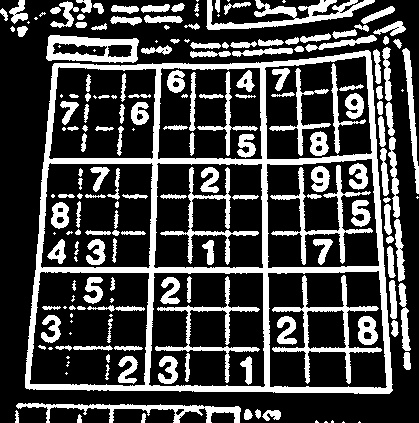
\includegraphics[width=\textwidth]{img/sht/input.jpeg}
      }
      \subcaptionbox{Wynik detekcji\label{fig:sht:output}}
      {
        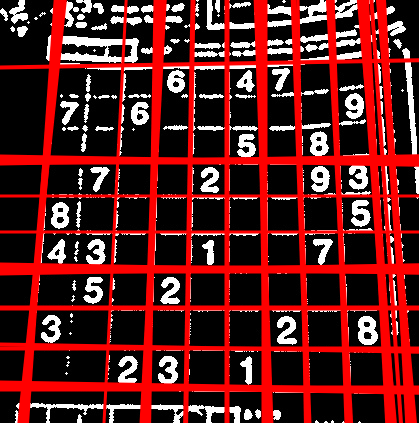
\includegraphics[width=\textwidth,trim=0 0 0 -1cm ]{img/sht/output.png}
      }%
      \end{minipage}%
  \hfill
  \begin{minipage}[c]{.475\linewidth}
    \subcaptionbox{Akumulator po głosowaniu\label{fig:sht:acc}}
      {
        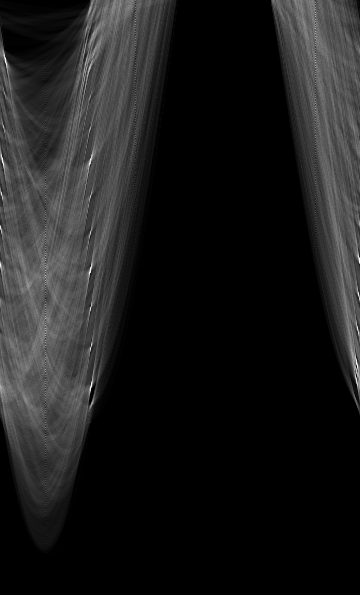
\includegraphics[width=\linewidth]{img/sht/equantial_acc.png}
      }%
  \end{minipage}%
  \caption{Wynik działania zaimplementowanego algorytmu SHT w~wariancie sekwencyjnym.}
  \label{fig:sht}
\end{figure}

\subsubsection{Circle Hough Transform}

Obraz testowy dla wariantu CHT przedstawiono na obrazie \ref{fig:cht:input}, a~wynik detekcji na \ref{fig:cht:output}. Poprzez rysowanie prostopadłych do kierunku krawędzi linii o~zakresie długości odpowiadającym długości wyszukiwanych promieni, w~procesie głosowania wygenerowany został akumulator przedstawiony na rysunku \ref{fig:cht:acc}. Jego rozmiar odpowiada rozmiarowi obrazu wejściowego, a~najjaśniejsze punkty są kandydatami na środki okręgów. Oprócz akumulatora dwuwymiarowego do detekcji promienia CHT wykorzystuje nieprzedstawiony tutaj akumulator jednowymiarowy, który bierze udział w~głosowaniu nad najlepszym promieniem. Dzieje się to osobno dla każdego kandydata na środek okręgu.

\begin{figure}
    \centering
    \begin{subfigure}{.475\linewidth}
          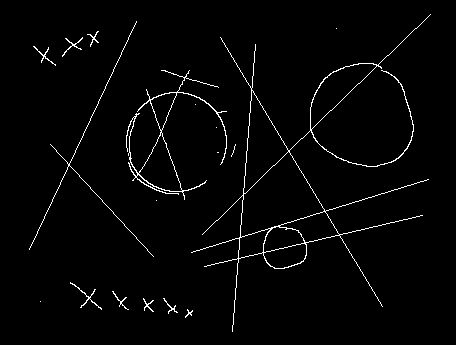
\includegraphics[width=\textwidth]{img/cht/input.png}
          \caption{Binarny obraz wejściowy}\label{fig:cht:input}
    \end{subfigure}%
    \hfill
    \begin{subfigure}{.475\linewidth}
      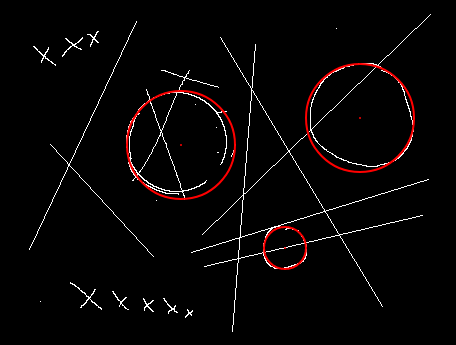
\includegraphics[width=\textwidth]{img/cht/output.png}
      \caption{Wynik detekcji}\label{fig:cht:output}
    \end{subfigure}% 
    \bigskip
    
    \begin{subfigure}{.475\linewidth}
      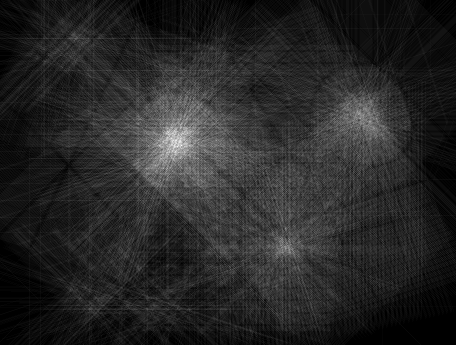
\includegraphics[width=\textwidth]{img/cht/sequential_acc.png}
      \caption{Akumulator po głosowaniu na środek okręgu}\label{fig:cht:acc}
    \end{subfigure}%
    \caption{Wynik działania zaimplementowanego algorytmu CHT w~wariancie sekwencyjnym.}
    \label{fig:cht}
  \end{figure}
  
\chapter{Implementacja i~wyniki pomiarów}
\label{sec:implementation}

\chapter{Podsumowanie}

Czy język JavaScript, jego ekosystem i~środowiska są przystosowane do wykonywania intensywnych obliczeń numerycznych? Czy asynchroniczny model wykonania wspiera, czy też przeszkadza w~wykonywaniu obliczeń? Czy środowiska zapewniają odpowiednie mechanizmy, aby wygodnie ładować dane, przyspieszać obliczenia oraz wyświetlać wyniki? Która z~metod akceleracji jest najbardziej wydajna oraz jak wygląda ich kompatybilność wśród środowisk? Czy istnieje możliwość bezkompromisowego utworzenia biblioteki kompatybilnej ze wszystkimi środowiskami? Na te i~inne pytania postarano się uzyskać odpowiedź w~tej pracy. Nie skorzystano w~tym celu z~syntetycznych testów wydajności środowisk języka JavaScript i~dostępnych metod akceleracji obliczeń oraz równoległej do nich analizy ich kompatybilności i~metod budowania bibliotek. Zamiast tego zastosowano podejście całościowe. Zaimplementowano algorytmy przetwarzania obrazów bazujące na transformacji Hough'a. Jest ona wykorzystywana w~algorytmach detekcji kształtów parametrycznych i~nieparametrycznych. W~zależności od kształtu i~wydajności powstały różne jej warianty. W~ramach tej pracy zaimplementowano wariant \textit{Standard} (Standard Hough Transform, SHT) i~\textit{Circle} (Circle Hough Transform, CHT) z~wykorzystaniem metody analizy gradientu do detekcji środków okręgów. Jako format eksportowanych bibliotek przyjęto moduły ES6 (ESModules).

Dla każdej z~analizowanych metod akceleracji przeprowadzono pomiary czasu wykonania we wszystkich udostępniających ją środowiskach. Do badanych środowisk należały przeglądarki internetowe Google Chrome i~Mozilla Firefox oraz środowiska serwerowe NodeJS i~Deno. Wszystkie z~nich korzystają z~V8 jako silnika języka JavaScript, co razem z~implementacją dla środowiska z~silnikiem SpiderMonkey - przeglądarki Mozilla Firefox, umożliwiło ich wzajemne porównanie. 

Jako definicję metody akceleracji przyjęto wszelkie działania, które potencjalnie mogą przyspieszyć wykonania algorytmu. Zaimplementowano algorytmy w~wariancie sekwencyjnym. Algorytm SHT dodatkowo został zaimplementowany z~wykorzystaniem stablicowanych wartości funkcji trygonometrycznych, co w~dużym stopniu zwiększyło wydajność. Do testów pozostałych metod akceleracji wykorzystano zatem trzy implementacje - dwie algorytmu SHT i~jedną CHT.

Podstawową metodą akceleracji była poprawa wydajności wykonania sekwencyjnego. Kolejną z~nich stanowiło wykorzystanie natywnych rozszerzeń środowiska NodeJS, których bazę stanowił kod C++. Następną z~nich było WebAssembly, którego bazę również stanowił kod w~języku C++ kompilowany do niskopoziomowego języka kompatybilnego z~wszystkimi środowiskami. Oprócz standardowej kompilacji, kod C++ skompilowano do kodu \textit{asm.js} oraz uruchomiono procesy automatycznej wektoryzacji wykonania podczas kompilacji do WebAssembly, aby wykorzystać wektorowe rejestry i~instrukcje procesora (SIMD). Przeprowadzono również kompilację po manualnej wektoryzacji kodu. Pierwszą z~metod wykorzystujących współbieżne wykonanie jest implementacja Worker'ów, gdzie zrównoleglone zostały iteracje najbardziej obciążonych pętli w~algorytmach. Ostatnią z~analizowanych metod było wykorzystanie potoku graficznego WebGL do przeprowadzenia masowo równoległych obliczeń.

Dla zaimplementowanych metod akceleracji podjęto próbę stworzenia biblioteki kompatybilnej ze wszystkimi środowiskami, co nie zawsze było możliwe. Zadbano jednak, aby każda z~bibliotek implementowała ten sam interfejs. Było to zapewnione przez transpilator języka TypeScript, w~którym to zaimplementowano wszystkie elementy bibliotek. Podczas transpilacji plików źródłowych do języka JavaScript, korzystał on z~tych samych symboli definiujących interfejs eksportowanych przez bibliotekę obiektów i~funkcji. Biblioteka zbudowana dla wariantu sekwencyjnego jest kompatybilna ze wszystkimi środowiskami, ponieważ opiera się tylko i~wyłącznie na standardowych mechanizmach języka JavaScript. Metoda wykorzystująca natywne rozszerzenia została zbudowana tylko dla środowiska NodeJS, które jako jedyne z~badanych udostępnia ją w~tej formie. Środowisko Deno również pozwala na zbudowanie i~wykonanie natywnych rozszerzeń, jednak bazą dla nich jest język Rust. Nie zostały one zaimplementowane, ponieważ implementacja algorytmów w~tym języku wykracza poza zakres tej pracy, która skupia się na bazowym kodzie w~języku C++. Dla tej metody, niezbędne było utworzenie warstwy powiązania, która zarządzała kopiowaniem danych oraz wywoływaniem właściwych funkcji. Narzędzie \textit{node-gyp} wraz z~Node-API niestety nie udostępniają automatycznych mechanizmów konwersji obiektów i~tablic z~języka JavaScript na ich odpowiedniki w~języku C++. Rodziło to konieczność ręcznego pobierania wartości do struktur na podstawie obiektu kontekstu wykonania. Kolejna zaimplementowana metoda wykorzystuje WebAssembly. Również tam niezbędne było utworzenie warstwy powiązania, jednak narzędzie \textit{Emscripten} udostępnia mechanizm automatycznej konwersji obiektów po zdefiniowaniu ich struktury, co zdecydowanie upraszcza proces implementacji. Jako, że proces inicjalizacji modułu WebAssembly musi odbyć się asynchronicznie, oraz nie zaimplementowano w~kodzie C++ mechanizmów łączenia zagnieżdżonych struktur, aby zapewnić domyślne wartości obiektom opcji, w~implementacji konieczne okazało się opakowanie modułu WebAssembly w~obiekt, który zajmuje się jego inicjalizacją oraz dostarcza domyślne dane opcji. Samo wywołanie funkcji implementowanych algorytmów odbywa się synchronicznie. Kompilacja z~użyciem narzędzia \textit{Emscripten}, aby uzyskać zakładany format modułu, wymaga użycia dodatkowych flag, co ma miejsce również w~przypadku wariacji formatów wyjściowych (\textit{asm.js}) i~używanych instrukcji (SIMD). Również i~w tym wypadku wszystkie środowiska, na których przeprowadzone zostały badania tej metody akceleracji, były kompatybilne z~tym samym kodem źródłowym.

Kompatybilności jednego kodu źródłowego ze wszystkimi środowiskami nie udało się uzyskać w~przypadku implementacji Worker'ów. Pomimo użycia biblioteki Comlink, która nałożyła warstwę abstrakcji ułatwiając komunikację głównego wątku z~Worker'ami, konieczne było utworzenie dwóch wersji kodu osobno dla środowisk przeglądarek internetowych i~osobno dla NodeJS. Środowisko Deno również wymagało utworzenia osobnej implementacji, ale w~odróżnieniu od pozostałych środowisk, gdzie biblioteka została zbudowana z~plików źródłowych, jest ono w~stanie wykonać pliki w~języku TypeScript. Konieczność budowania wielu wersji biblioteki wymusza niekompatybilny pomiędzy środowiskami przeglądarek, Deno i~NodeJS interfejs obsługi Worker'ów. Dlatego też, aby zapewnić możliwość współdzielenia kodu samego algorytmu dla tej metody akceleracji, niezbędne jest użycie adapterów oraz zbudowanie osobnych wersji biblioteki dla każdego ze środowisk.

Kolejną metodą niekompatybilną ze wszystkimi badanymi środowiskami jest wykorzystanie GPGPU poprzez użycie WebGL API, czyli potoku graficznego do obliczeń ogólnego przeznaczenia. Jest ona możliwa do wdrożenia natywnie jedynie w~przeglądarkach internetowych. W~NodeJS istnieje konieczność z~zainstalowania zewnętrznej implementacji WebGL, a~środowisko Deno nie wspiera jej wcale. Metoda ta, w~przeciwieństwie do użycia GPGPU w~przystosowanych do tego rozwiązaniach, nie umożliwia interakcji z~pamięcią współdzieloną pomiędzy wątkami, a~wynikiem obliczeń jest tylko kolor piksela. Jako liczba może być on jednak dowolnie interpretowany. Metoda ta, pomimo swoich wad i~wykorzystania potoku niezgodnie z~jego przeznaczeniem, może przynieść zdecydowaną poprawę wydajności algorytmów. Muszą one jednak być podatne na masowe zrównoleglenie oraz nie korzystać z~pamięci współdzielonej. Przykładem najprostszego z~nich może być mnożenie macierzy, czy operacja splotu. Dołączona biblioteka \textit{gpu.js}, służąca do obsługi interakcji z~potokiem graficznym, transpiluje kod JavaScript na kod programu \textit{Fragment Shader} potoku graficznego. Proces budowania musi uwzględniać mechanizmy minifikacji kodu, ponieważ mogą one interferować z~ową transpilacją i~produkować kod i~jego konstrukcje niezrozumiałe przez bibliotekę \textit{gpu.js}.


\newcommand{\comma}{, }
\begin{table}
    \label{tab:envs}
    \caption{Comparison of implemented methods in analyzed environments. The general comparison was done using Chrome as a reference point and geometric mean for times comparable with Chrome.}

    \begin{tabularx}{\linewidth}{X r r r r}%
        \hline
                                 & \multicolumn{4}{c}{\bfseries Execution time[ms]}                                                             \\
        \bfseries Method         & \bfseries Chrome                                 & \bfseries Firefox     & \bfseries Node  & \bfseries Deno

        \csvreader[
            head to column names,
            before first line=                                                                                                                  \\\hline,
            late after line=                                                                                                                    \\,
            late after last line=                                                                                                               \\\hline
        ]{../../benchmark/environments/envs.csv}{}% use head of csv as column names
        {
        \name\                   & \chrome\ (\chromeF)                              & \firefox\ (\firefoxF) & \node\ (\nodeF) & \deno\ (\denoF)
        }% specify your coloumns here 
        \bfseries Geometric mean &
        \csvreader[
            head to column names,
            late after last line=                                                                                                               \\\hline

        ]{../../benchmark/environments/geoMeans.csv}{}% use head of csv as column names
        {
        (\chrome)                & (\firefox)                                       & (\node)               & (\deno)
        }% specify your coloumns here 
    \end{tabularx}

\end{table}


W tabeli \ref{tab:envs} przedstawiono podsumowanie czasów wszystkich pomiarów wydajności dla wartości próbkowanie $S_\theta=1$ dla wariantu SHT algorytmu i~współczynnikiem maksymalnego promienia $n=10$ dla CHT. Wykonanie dla algorytmu CHT z~metodą WebGL nie zostało uwzględnione, ponieważ w~implementacji wystąpiły błędy, co opisano w~sekcji \ref{sec:cht-gpu}. W~ogólnym podsumowaniu najbardziej wydajnym środowiskiem okazało się Google Chrome. Kolejnymi środowiskami pod względem wydajności są NodeJS i~Deno, których wydajność jest porównywalna. Najwolniejszym ze środowisk jest przeglądarka Mozilla Firefox. Osiągnęła ona wyniki porównywalne z~Google Chrome jedynie w~przypadku akceleracji z~użyciem WebGL, gdzie ciężar obliczeń oddelegowany jest do GPU, a~przeglądarka odpowiedzialna jest za przekazanie danych i~skompilowanie programów shader'ów.

Najlepszą z~metod, których bazę stanowił kod w~C++, jest użycie natywnych rozszerzeń w~środowisku NodeJS. WebAssembly, również przynosi poprawę wydajności we wszystkich środowiskach w~porównaniu do wykonania sekwencyjnego. Wykorzystanie automatycznej wektoryzacji kodu, aby wykorzystać instrukcje i~rejestry wektorowe nie przyniosło rezultatów w~żadnym środowisku w~porównaniu do zwykłego WebAssembly. Manualna wektoryzacja, która wymagała modyfikacji kodu C++ i~użycia specjalnych instrukcji operujących na tych rejestrach, przyniosła poprawę wydajności dla algorytmów SHT, którego dane wejściowe wymuszały większą intensywność obliczeń w~modyfikowanych pętlach. Dla algorytmów CHT manualna wektoryzacja nie przyniosła żadnych rezultatów, bądź nawet spowolniła wykonanie. Pozwala to wysnuć wniosek, że manualna wektoryzacja dołożyła czas związany z~jej obsługą, który zrekompensowany został poprzez intensywne jej wykorzystanie, co miało miejsce dla testów algorytmów SHT i~nie dla CHT. Metoda wykorzystujące \textit{asm.js} jako jedyna nie przyniosła poprawy wydajności. Spowodowane to być może sposobem budowania biblioteki z~kodem \textit{asm.js}, który uniemożliwił prawidłową jego interpretacje przez przeglądarki, ale również to, że \textit{asm.js} jest natywnie wspierany - kompilowany Ahead-of-Time jedynie w~przeglądarce Mozilla Firefox.

Największe przyspieszenie umożliwiło wykorzystanie Worker'ów oraz WebGL z~oczywistą przewagą tego drugiego. Wyniki te nie dziwią, ponieważ naturalnym jest osiągnięcie lepszych wyników wykonując obliczenia równolegle. Przewaga WebGL jest o~tyle specyficzna, że implementowany algorytm musi dać się masowo zrównoleglić bez wpływu na opisane wcześniej wady tej metody, podczas gdy nie trzeba się o~to martwić w~przypadku Worker'ów. 

Badania te pozwalają stwierdzić, że środowiska języka JavaScript są gotowe, aby zapewnić wysoką wydajność obliczeń numerycznych. Wszystkie zaimplementowane metody akceleracji poza \textit{asm.js} zmniejszyły lub nie zmieniły czasu wykonania w~ramach środowiska. Dalsze prace nad testowaniem wydajności mogą sprawdzać działanie hybrydowych metod akceleracji, czego przykładem może być zastosowanie Worker'ów, a~w nich WebAssembly. Dodatkowo można zastosować podejście SIMD. Niezbędna jest również analiza implementacji algorytmu CHT, który osiągnął niewspółmiernie długie czasy wykonania podczas testów metody opartej na WebGL. Na podstawie ogólnego rozeznania w~możliwościach każdej z~metod akceleracji, implementacji algorytmów oraz sposobów budowania bibliotek, możliwym staje się wybór interesujących elementów składowych algorytmów, ich ekstrakcja i~izolowane testy syntetyczne, co może również być przedmiotem dalszych badań. Możliwym ich kierunkiem z~pewnością powinna stać się również implementacja i~analiza wydajności tych algorytmów dla akceleracji obliczeń z~użyciem WebGPU i~sprawdzenie, czy i~w jakim stopniu rozwiązuje on problemy wynikające z~niedoskonałości metody opartej na WebGL.

JavaScript, pomimo bycia rozwiniętym językiem z~bogatym ekosystemem, nie pozwala na budowę szeroko kompatybilnych bibliotek ze względu na różnice wśród środowisk i~ich różną specyfikę. Do najszybszych obliczeń, co pokazują przeprowadzone testy, i~prezentacji ich wyników najlepszym środowiskiem jest przeglądarka Google Chrome. Jednak konieczność budowania, trudność w~prototypowaniu rozwiązań oraz bycie środowiskiem odizolowanym od systemu operacyjnego skutecznie powstrzymało rozwój jego zastosowania w~obszarze obliczeń numerycznych. Środowiska serwerowe leżą po drugiej stronie barykady. Mają możliwość bezpośredniej interakcji z~systemem operacyjnym. Pomiędzy nimi występują jednak braki w~kompatybilności, czego przykładem jest interfejs obsługi Worker'ów w~NodeJS i~Deno. Prezentacja wyników w~formie graficznej wymaga wygenerowanie ich i~wyświetlenie w~postaci strony internetowej lub zapisania plików, podczas gdy w~języku Python biblioteki są w~stanie wyświetlić wyniki w~osobnych oknach.

Różnice środowisk, ich wzajemne wady i~zalety, oraz oczywiście docelowe zastosowanie samego języka były przyczyną powolnej ewolucji ekosystemu bibliotek, który jest w~tej chwili głównym hamulcem w~rozwoju tej gałęzi obliczeń w~języku JavaScript. Bibliotek jest mało, są mało popularne, co przekłada się na tempo ich rozwoju i~podążania za wydajnością i~kompatybilnością ze środowiskami. Jednak jak to zawsze bywa, najtrafniejszą odpowiedzią na większość pytań z~początku tego rozdziału będzie: \textit{To zależy}. W~zależności od wymaganych opóźnień i~zakładanego obciążenia konsekwencje asynchroniczności oraz braku bezpośredniego wsparcia dla wątków mogą stanowić problem. W~zależności od wymaganego środowiska dla wdrożenia aplikacji oraz zakładanego formatu prezentacji wyników środowisko przeglądarki może okazać się odpowiednie. W~zależności od implementowanego algorytmu będzie możliwe zastosowanie wybranych metod akceleracji. Pewnym jest jednak, że bezkompromisowe utworzenie biblioteki bez zważania na stosowana metodę akceleracji jest niemożliwe. Dla całego spektrum rozważań na temat algorytmów i~języków implementujących obliczenia numeryczne, te o~przystosowaniu środowisk języka JavaScript stanowią jedynie ich niewielką część. Powinny być one bowiem skoncentrowane w~pierwszej kolejności na złożoności obliczeniowej samych algorytmów, co jest najlepszym sposobem poprawy ich wydajności.

\clearpage




%\bibliographystyle{plalpha}
\bibliographystyle{abbrv}
% \bibliographystyle{plain}

%Warning: References should be collected in a separate file. You can use the programm JabRef for editing. 
%         But please remember, that not all JabRef types of entries are supported by BibTeX.
%         File name below is given without extenion 
%         (here BibTeX will look for "bibiography.bib" in the main directory)
\setlength{\bibitemsep}{2pt} % introduced to make smaller seps between bibliographic items
\bibliography{bibliography}

\appendix
\chapter{Opis załączonej płyty CD/DVD}
Dołączona płyta zawiera wszystkie pliki wykorzystane do stworzenia projektu, dokumentacji i~niniejszej pracy. Na płycie znajduje się cała zawartość projektu zaimplementowanego w~strategii \textit{monorepo} i~w katalogu głównym znajdują się pliki odpowiedzialne za jej obsługę.  Pozostałe pliki podzielono na następujące katalogi:

\begin{itemize}
    \item \texttt{.vscode} - ustawienia środowiska VsCode,
    \item \texttt{benchmark} - wyniki testów wydajności w~formacie \texttt{*.csv},
    \item \texttt{docs} - notatki oraz treść i~materiały niniejszej pracy,
    \begin{itemize}[topsep=0pt]
        \item[\textbullet] \texttt{notes} - notatki
        \item[\textbullet] \texttt{out} - pliki będące wynikiem kompilacji plików źródłowych pracy
        \begin{itemize}[topsep=0pt]
            \item[\textbullet] \texttt{W04N\_241292\_2022\_praca magisterska.pdf} - plik PDF z~zawartością pracy
        \end{itemize}
        \item[\textbullet] \texttt{src} - pliki źródłowe pracy
    \end{itemize} 
    \item \texttt{packages} - zbiór pakietów \textit{monorepo}
    \begin{itemize}[topsep=0pt]
        \item[\textbullet] \texttt{benchmark} - Biblioteka \textit{benchmark}
        \item[\textbullet] \texttt{cpp-sequential} - Implementacja metody sekwencyjnej w~C++
        \item[\textbullet] \texttt{frontend} - Rzeczywisty przykład użycia
        \item[\textbullet] \texttt{js-benchmarks} - Przeprowadzanie pomiarów wydajności
        \item[\textbullet] \texttt{js-gpu} - Implementacja metody WebGL
        \item[\textbullet] \texttt{js-sequential} - Implementacja metody sekwencyjnej w~JavaScript
        \item[\textbullet] \texttt{js-workers} - Implementacja metody Workers
        \item[\textbullet] \texttt{meta} - Typy języka TypeScript współdzielone pomiędzy implementacje
        \item[\textbullet] \texttt{node-cpp-sequential} - Implementacja metody Native C++ Addon w~NodeJS
        \item[\textbullet] \texttt{test-simple} - Strona testowa dla implementowanych metod
        \item[\textbullet] \texttt{wasm-sequential} - Implementacja metody WASM oraz jej wariantów
    \end{itemize} 
    \item \texttt{test} - zbiór testowych obrazów,
\end{itemize}

%\include{appendixB}

%%Uncomment the lines below, if you want to use index
%%\chapterstyle{noNumbered}
%%\phantomsection 
%%\addcontentsline{toc}{chapter}{Index}
%%\printindex


\end{document}
